\documentclass{wissdoc}

%% --------------------
%% |     Packages     |
%% --------------------

\usepackage[utf8]{inputenc}

% Weitere packages: (Dokumentation dazu durch "latex <package>.dtx")

%\usepackage{bibgerm}
%\usepackage[backend=biber]{biblatex} 
\usepackage{csquotes} 
\usepackage{tabularx}
\usepackage{booktabs}
\usepackage{multirow}
%\usepackage{tocbibind}
\usepackage{siunitx}
\usepackage{xcolor}
\usepackage{textcomp}
\usepackage{listings}
\usepackage{newfloat,caption}
\usepackage{subcaption}
\usepackage{footnote}
\usepackage{rotating}
\usepackage{pgfplots}
\usepackage{pgfplotstable}
\usepackage{url}
\usepackage{boxhandler}
\usepackage{tabu}
\usepackage{amssymb}
% \usepackage{subfig}
\usepackage{caption}
\usepackage{subcaption}
%\usepackage[plainpages=true]{hyperref}
\usepackage[space]{grffile}
\usepackage{pdfpages}
%\usepackage[numbers,sort&compress]{natbib}
\usepackage[backend=bibtex,natbib=true,hyperref=true,doi=false,url=false]{biblatex}
% \usepackage{varioref}
% \usepackage{verbatim}
\usepackage{float}    %z.B. \floatstyle{ruled}\restylefloat{figure}
%\usepackage[hidelinks]{hyperref}
% \usepackage{subfigure}
% \usepackage{fancybox} % für schattierte,ovale Boxen etc.
% \usepackage{tabularx} % automatische Spaltenbreite
% \usepackage{supertab} % mehrseitige Tabellen
% \usepackage[svnon,svnfoot]{svnver} % SVN Versionsinformation 

% My packages
\usepackage{graphicx}

\usepackage{minted}
\usepackage{svg}

%% --------------------
%% |     Settings     |
%% --------------------

% Settings: Titlepage, Comments, etc.
\pgfplotsset{compat=newest}

% Settings for Titlepage
\hypersetup{
	colorlinks,
  citecolor=black,
  filecolor=black,
  linkcolor=black,
  urlcolor=black,
 pdfauthor={FirstName LastName},
 pdftitle={Title of Thesis}
 pdfsubject={Not set},
 pdfkeywords={Not set}
}
% \DeclareFloatingEnvironment[fileext=frm,placement={!ht},name=Listing,within=section]{listing}

% Print URLs not in Typewriter Font
\def\UrlFont{\rm}

\newcommand{\specialcell}[2][c]{%
  \begin{tabular}[#1]{@{}c@{}}#2\end{tabular}}

\newcommand\todo[1]{\textcolor{red}{TODO: #1}}

\newcommand\hlcode[1]{\textcolor{red}{#1}}

\newcommand\citeable[1]{\textcolor{green}{\hl{citeable: #1}}}

\newcolumntype{\$}{>{\global\let\currentrowstyle\relax}}
\newcolumntype{^}{>{\currentrowstyle}}
\newcommand{\rowstyle}[1]{\gdef\currentrowstyle{#1}%
  #1\ignorespaces
}

% Comments
\newif\ifcomment
%\commenttrue

% Leerseite ohne Seitennummer, nächste Seite rechts
\newcommand{\blankpage}{
 \clearpage{\pagestyle{empty}\cleardoublepage}
}

% \lstset{%
%   language = Octave,
%   backgroundcolor=\color{white},   
%   basicstyle=\footnotesize\ttfamily,       
%   breakatwhitespace=false,         
%   breaklines=true,                 
%   captionpos=b,                   
%   commentstyle=\color{gray},    
%   deletekeywords={...},           
%   escapeinside={\%*}{*)},          
%   extendedchars=true,              
%   frame=single,                    
%   keepspaces=true,                 
%   keywordstyle=\color{orange},       
%   morekeywords={*,...},            
%   numbers=left,                    
%   numbersep=5pt,                   
%   numberstyle=\footnotesize\color{gray}, 
%   rulecolor=\color{black},         
%   rulesepcolor=\color{blue},
%   showspaces=false,                
%   showstringspaces=false,          
%   showtabs=false,                  
%   stepnumber=2,                    
%   stringstyle=\color{orange},    
%   tabsize=2,                       
%   title=\lstname,
%   emphstyle=\bfseries\color{blue}%  style for emph={} 
% } 

% %% language specific settings:
% \lstdefinestyle{Arduino}{%
%     language = Octave,
%     keywords={void, int boolean},%                 define keywords
%     morecomment=[l]{//},%             treat // as comments
%     morecomment=[s]{/*}{*/},%         define /* ... */ comments
%     emph={HIGH, OUTPUT, LOW}%        keywords to emphasize
% }

% Bibliography
\addbibresource{bib/references.bib}

%% --------------------------------------------------------------------------------
%% |                           BEGINNING OF DOCUMENT                              |
%% --------------------------------------------------------------------------------
\begin{document}

%% ----------------------
%% |     Title Page     |
%% ----------------------
\frontmatter
\pagenumbering{roman}
\ifnotdraft{
 
\includepdf[pages=-]{BA_Melnic_Alexandr_Titelseiten.pdf}
}

%% ----------------------------
%% |     Table of Content     |
%% ----------------------------

\ifnotdraft{
\pagenumbering{roman}
{\parskip 0pt\tableofcontents} % toc bitte einzeilig
\listoffigures
\listoftables
}
\cleardoublepage
{\pagestyle{empty}
~
\cleardoublepage}
%\thispagestyle{empty}

%% ------------------
%% |     Content    |
%% ------------------

\graphicspath{{src/}}

\mainmatter
\pagenumbering{arabic}

\chapter*{Abstract}
\label{ch:Abstract}
%% ==============================
English version of the Kurzfassung. Try to stay within 500 words (single page).

\chapter{Introduction}
\label{ch:Introduction}

One of the most occurring temporomandibular joint (TMJ) dysfunction is bruxism. Altough debatable some studies suggest prelevance in up to 15\% of children and in as many as 96\% of adults \cite{thompson1994treatment}.

It can manifest itself trhoughout the day or night or both. 

We diferentiate between ``Awake Bruxism`` (AB) or ``Sleep Bruxism`` (SB) based on the time-period when it occurs. The masticatory muscle contraction and contraction types are also different from person to person and between AB and SB

In esence bruxism is a set of patterns of movements of the jaw with different periodicity, force and duration. Some of such patterns include clenching, grinding and sliding of the jaw.

Bruxism can be hard to diagnose

80\% of bruxism episodes are not accompanied by noise \cite{shetty2010bruxism}

80\% of bruxers are not aware of their condition \cite{thompson1994treatment}

If not treated bruxism can cause to teeth fracture, headache or masticatory muscle problems.

The ultimative diagnose of the bruxism is usually done in a controlled lab environment during a sleep study. This tends to be very expensive and impractical in assesting of the AB.

A more convinient and universal way would be the use of one or a combination of affordable wearable devices. The primary purpose of such wearables can be completly different, but the internal sensors can be repurposed and trained to classify jaw movements.

Based on previous research in the field, it was interesting to compare different wearables in the same experiment environment.
\chapter{Background \& Related Work}
\label{ch:Background}

While researching for previews attempts to classify bruxism, the scope was enlarged to include attempts to classify jaw movements in general.

76\% on grinding and 73\% on clenching detection accuracy achieved by \cite{bondareva2021earables} using earphones (eSense earables). 
94\% on chewing detection accuracy achieved by \cite{lotfi2020comparison} using earphones (eSense earables).
1\% to 4\% error rate on chewing detection accuracy achieved by \cite{lotfi2020comparison} using earphones (eSense earables).


 F1-scores on grinding up to 0.9 using around-the-ear EEG electrodes \cite{Knierim2021}
 
 87.6\% detection accuracy for face-related movements using barometer placed in earphones \cite{Ando2017}
 
 Reliable detection of up to 7 jaw-gestures using earphone speakers as microphones and recording vibrations propagated to the ear-canal \cite{Prakash2020}
 
 Recognition of 13 teeth tapping gestures with 90.9\% accuracy using custom-built ear-pieces with IMU on each side of the user jaw \cite{Sun2021}
 
 100\% detection accuracy of bruxism using EMG signals. \cite{Sonmezocak2021}
 
 
\newcommand{\usedspecs}[5]{
\begin{table}[h!]
\centering
\begin{tabular}{|c||c|} 
 \hline
 Interface & #1 \\
 \hline
 Sample rate & #2 \\ 
 \hline
 Data & #3 \\ 
 \hline
\end{tabular}
\caption{#4. Used technical specifications}
\label{table:#5_specs}
\end{table}
}

\chapter{Implementation}
\label{ch:Implementation}

\section{Hardware}
\label{sec:hardware}

Based on previous research a set of devices and sensors was selected. The selection was done with a goal in mind: to utilize the maximum of the \emph{available space} on a human head and neck. Assuming that those surfaces will allow the recording of the vibrations and movements generated by the jaw movements. 

A Raspberry Pi 3 B+ (RPI) was used a the central processing unit. It has a Bluetooth antenna as well as a variety of wired connectivity options to ease the build of this prototype. As discussed later in \ref{sec:software} the RPI was used not only for the data collection, but as well for the real-time data visualization. The RPI had some hardware limitations to read the raw data directly from some of the sensors. It was solved by using external microcontrollers, see \ref{subsub:bno}, \ref{subsub:emg}.

\subsection{Peripherals}

\begin{table}[h!]
\centering
\begin{tabular}{|>{\raggedright}m{0.25\linewidth}|>{\centering}m{0.1\linewidth}|m{0.3\linewidth}|m{0.25\linewidth}|} 
 \hline
 Device & Amount & Sensor & Area of contact \\ [0.5ex] 
 \hline\hline
 eSense earables \ref{subsub:esense} & 2 & 6 DOF IMU & In ear \\ 
 \hline
 Arduino BNO055 \ref{subsub:bno} & 2 & 9 DOF IMU & Back side of the jaw \\ 
 \hline
 Olimex EMG-Shield & 4 & Electromyography (EMG) & Masseter and temporalis muscles \\ 
 \hline
 Throat microphone & 1 & Vibration sensor & Neck \\ 
 \hline
 Grove GSR & 1 & Galvanic skin response (GSR) & Index and middle finger \\ 
 \hline
\end{tabular}
\caption{Used sensors}
\label{table:used_sensors}
\end{table}

\subsubsection{eSense earables}
\label{subsub:esense}

\begin{figure}[h!]
\centering
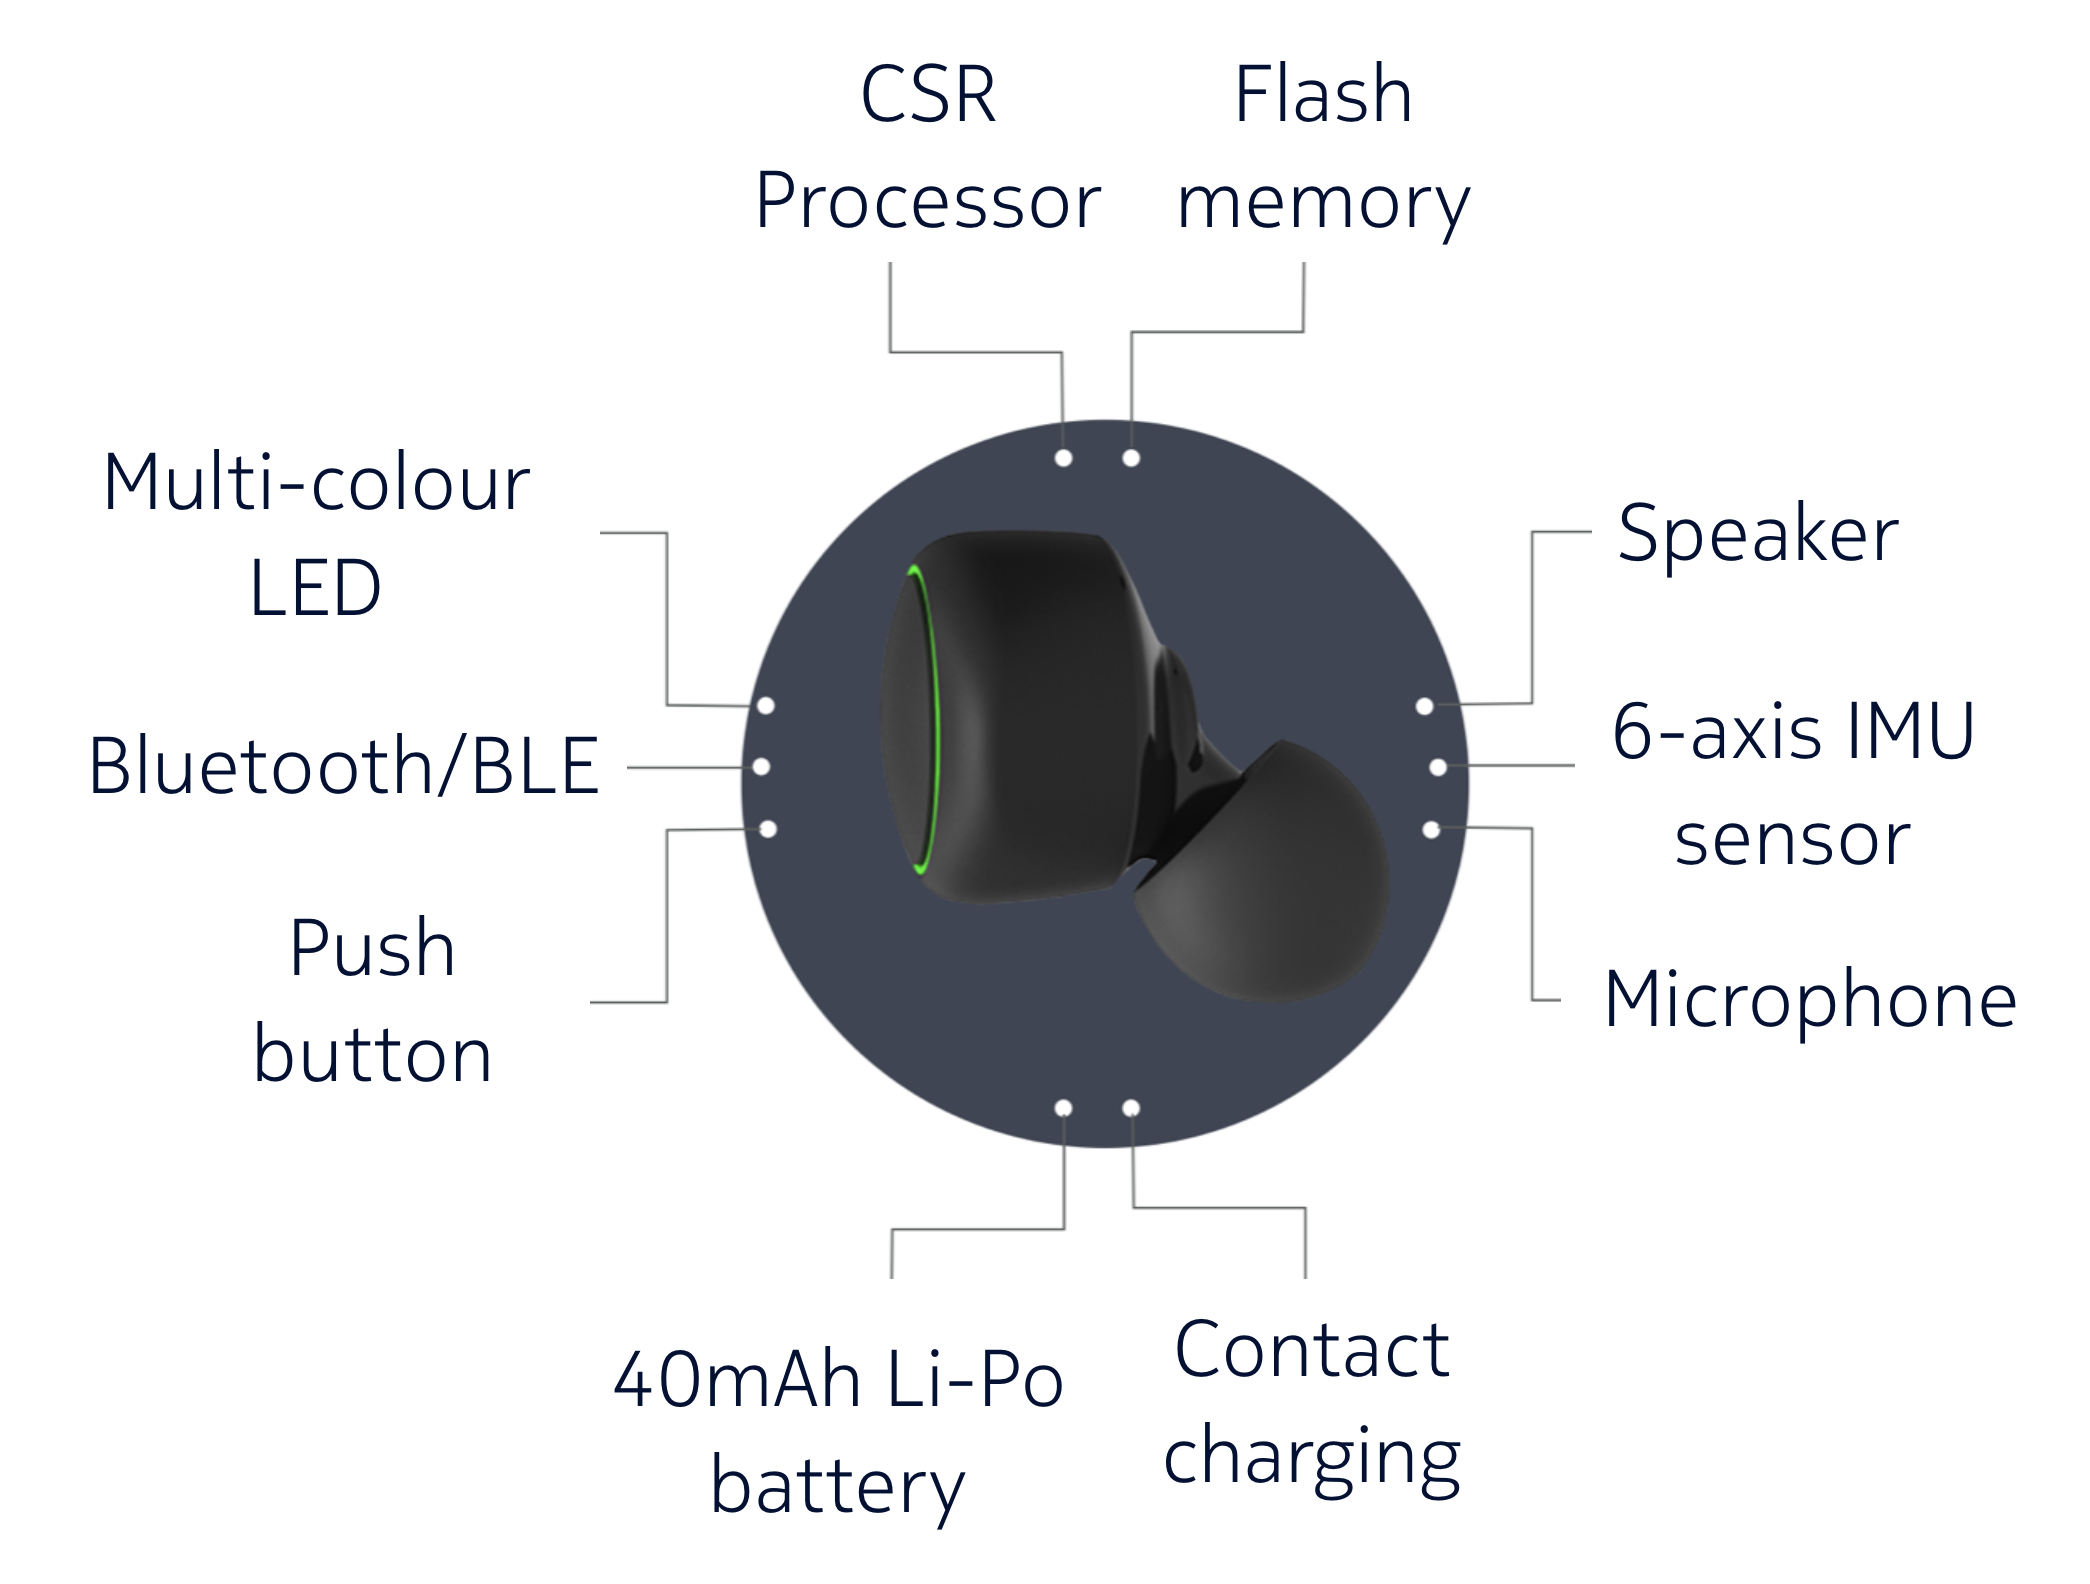
\includegraphics[width=0.5\textwidth]{src/media/hardware/esense.png}
\caption{eSense earable \cite{min2018exploring, kawsar2018earables}}
\label{image:esense}
\end{figure}

The eSense earables are a pair of true wireless earphones. The data we are interested in is the 6 DOF IMU located only in the left earpiece only. Because of this limitation two left earpieces were used. Even though the left and right ear pieces are not interchangeable, the participants in the user study didn't notice any difference in the fit in the right ear.

The default frequency of sending of the IMU data is set to 10Hz. Because in this research we are interested solely in the readings from the IMU (no audio playback) it is possible to increase the frequency to up to 100Hz \cite{esense_ble_specification}.

The connection was done directly with the RPI by using a python package called \texttt{bleak}.

\usedspecs{BLE}{100Hz}{Accelerometer \& gyroscope}{eSense earable}{esense}

\subsubsection{Arduino BNO055}
\label{subsub:bno}

\begin{figure}[h!]
\centering
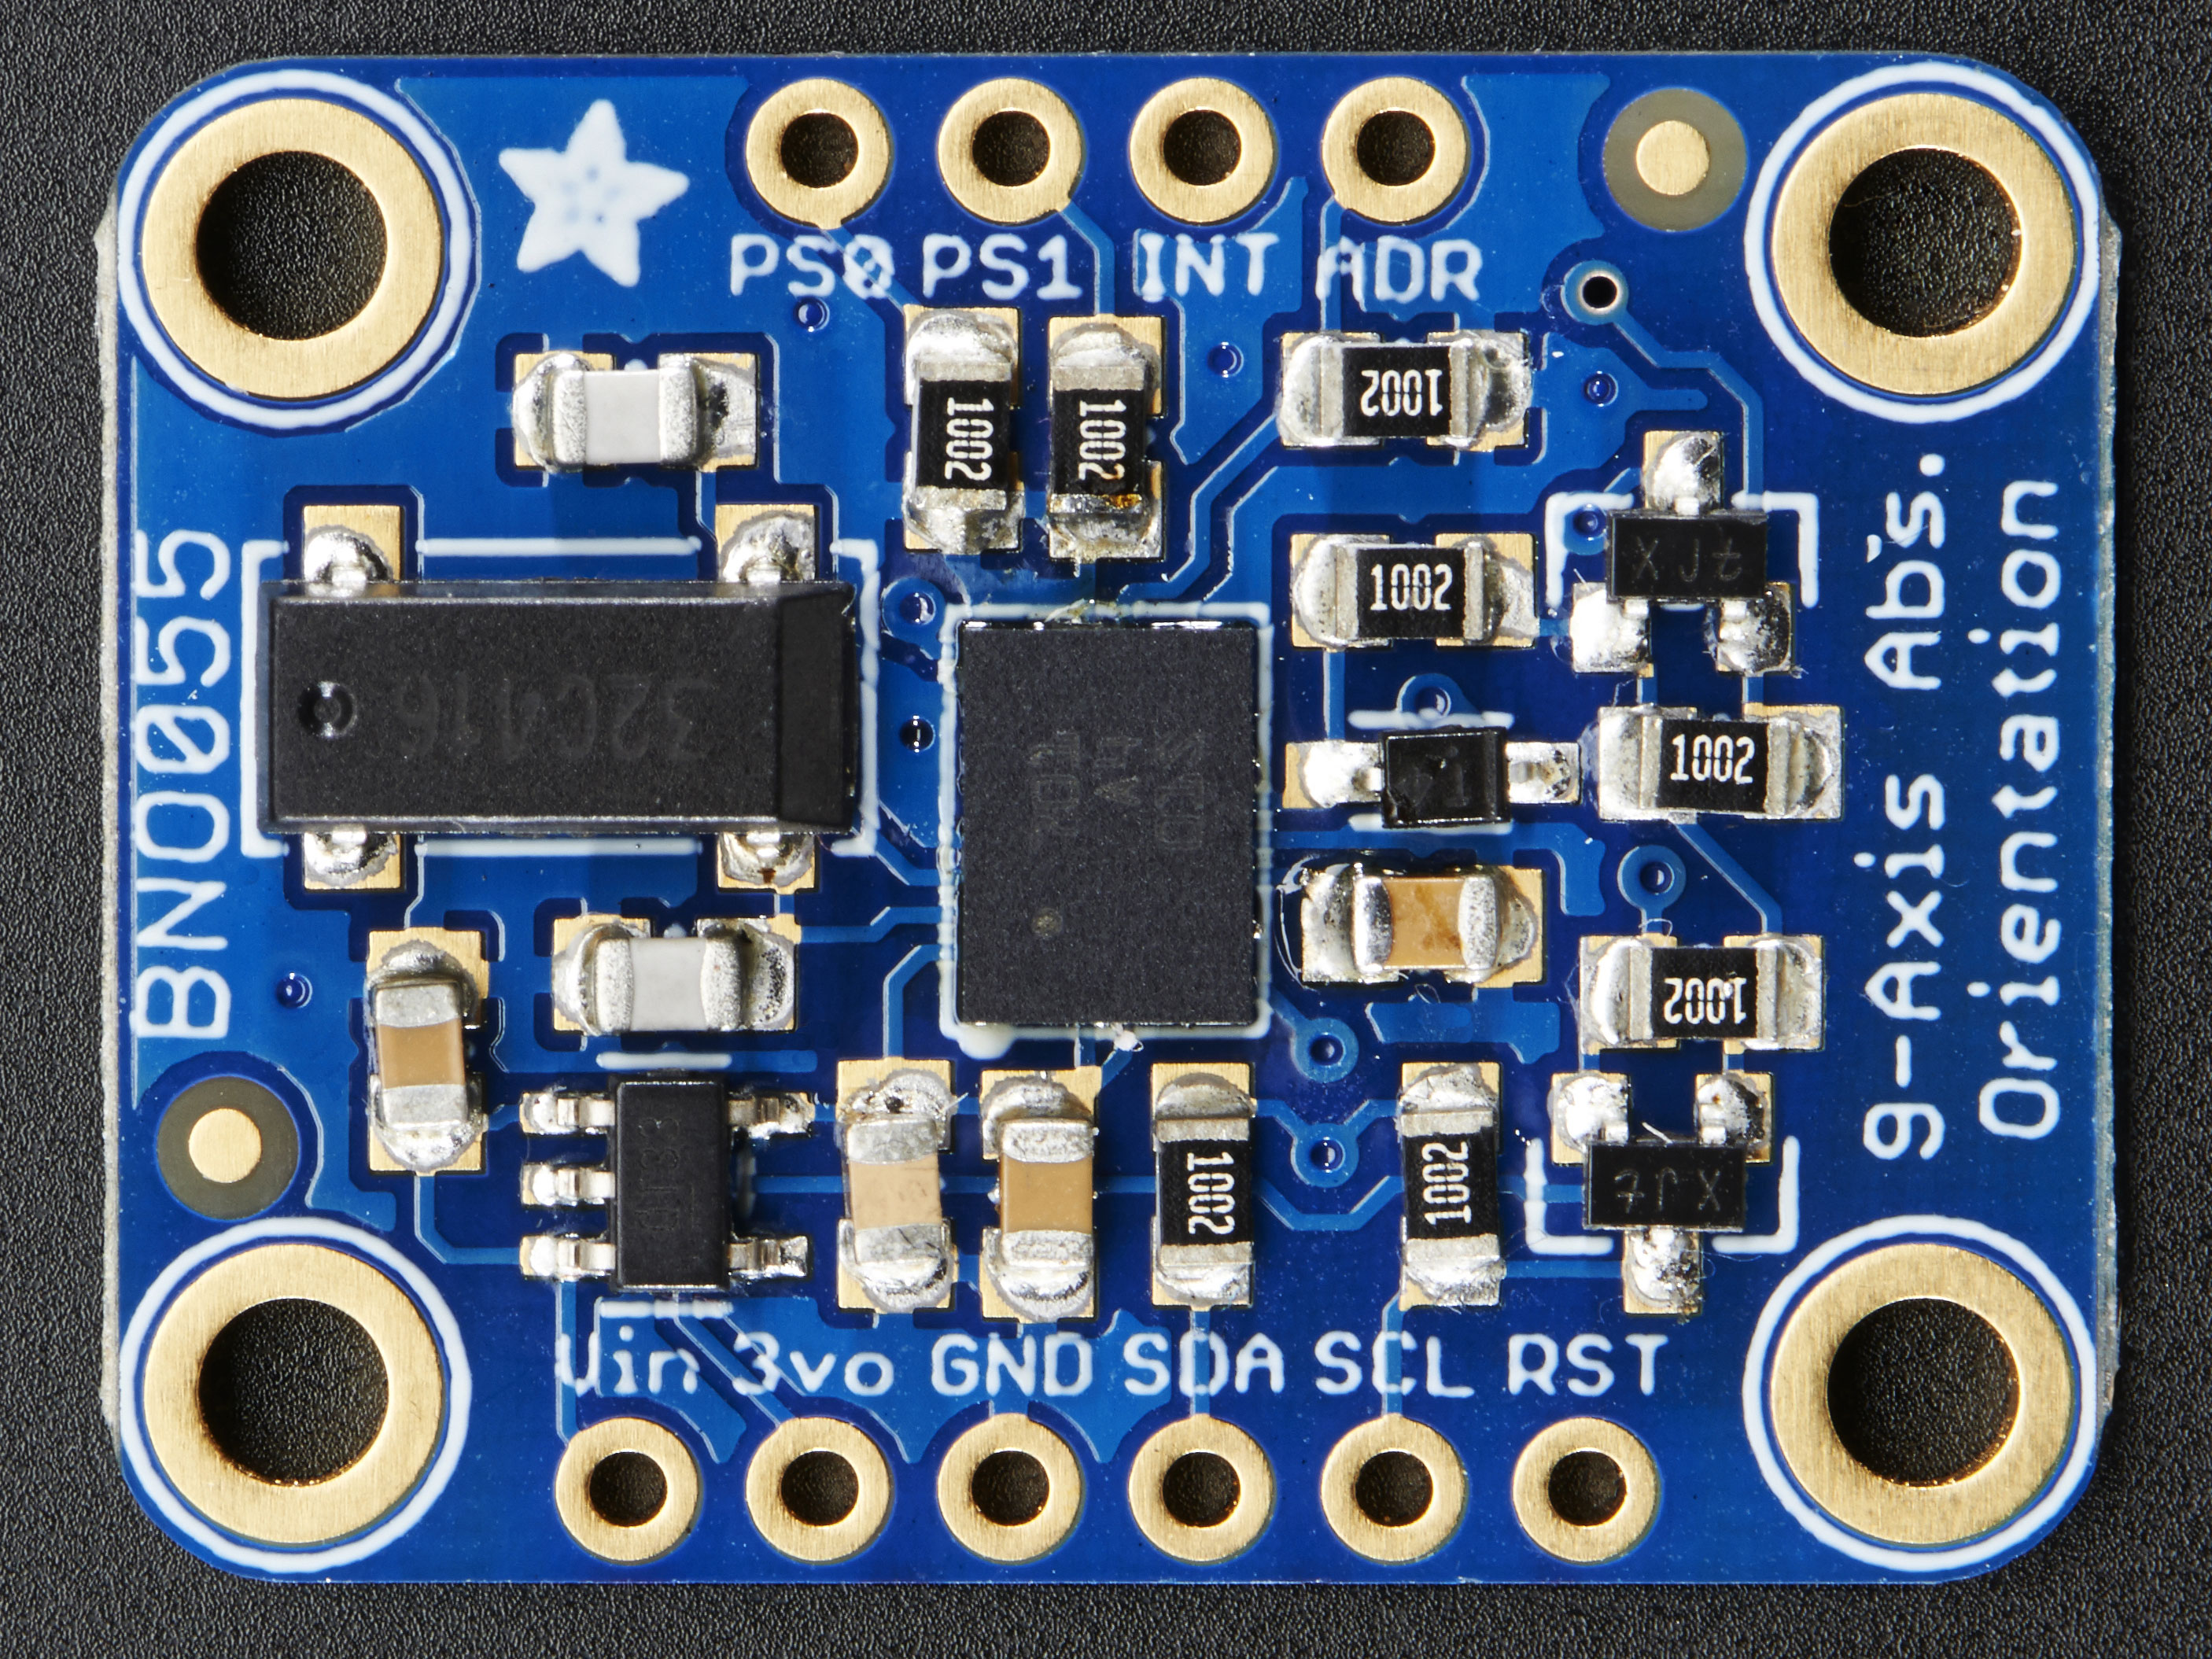
\includegraphics[width=0.5\textwidth]{src/media/hardware/bno.jpg}
\caption{Arduino BNO055 breakout board}
\label{image:bno}
\end{figure}

This (fig. \ref{image:bno}) small breakout board from Arduino has a BNO055, a 9 DOF IMU with sensor fusion on the chip. The fastest of the available protocols for data transmission is I2C. Fortunately the BNO055 has an \texttt{ADR} pin, which if set to high will change its I2C address. It allows the communication with both of the used BNO055s over the same I2C bus.

Even though the RPI has pins for the I2C communication, it doesn't support clock stretching. Using the RPI the collected data was at a much lower frequency (around 30Hz) and generally the connection was unreliable.

After testing different microcontrollers, the decision was made to use the Adafruit Feather HUZZAH ESP8266 board, to read the raw data from the BNO055s and then send it directly to the RPI. Because the RPI couldn't handle reliably more than 2 BLE connections at the same time, the IMU data was transmitted over the Serial Protocol (USB).

\usedspecs{Serial}{100Hz}{Accelerometer \& gyroscope \& quaternion}{Arduino BNO055 in combination with Feather Huzzah}{esense}

\begin{figure}[h!]
\centering
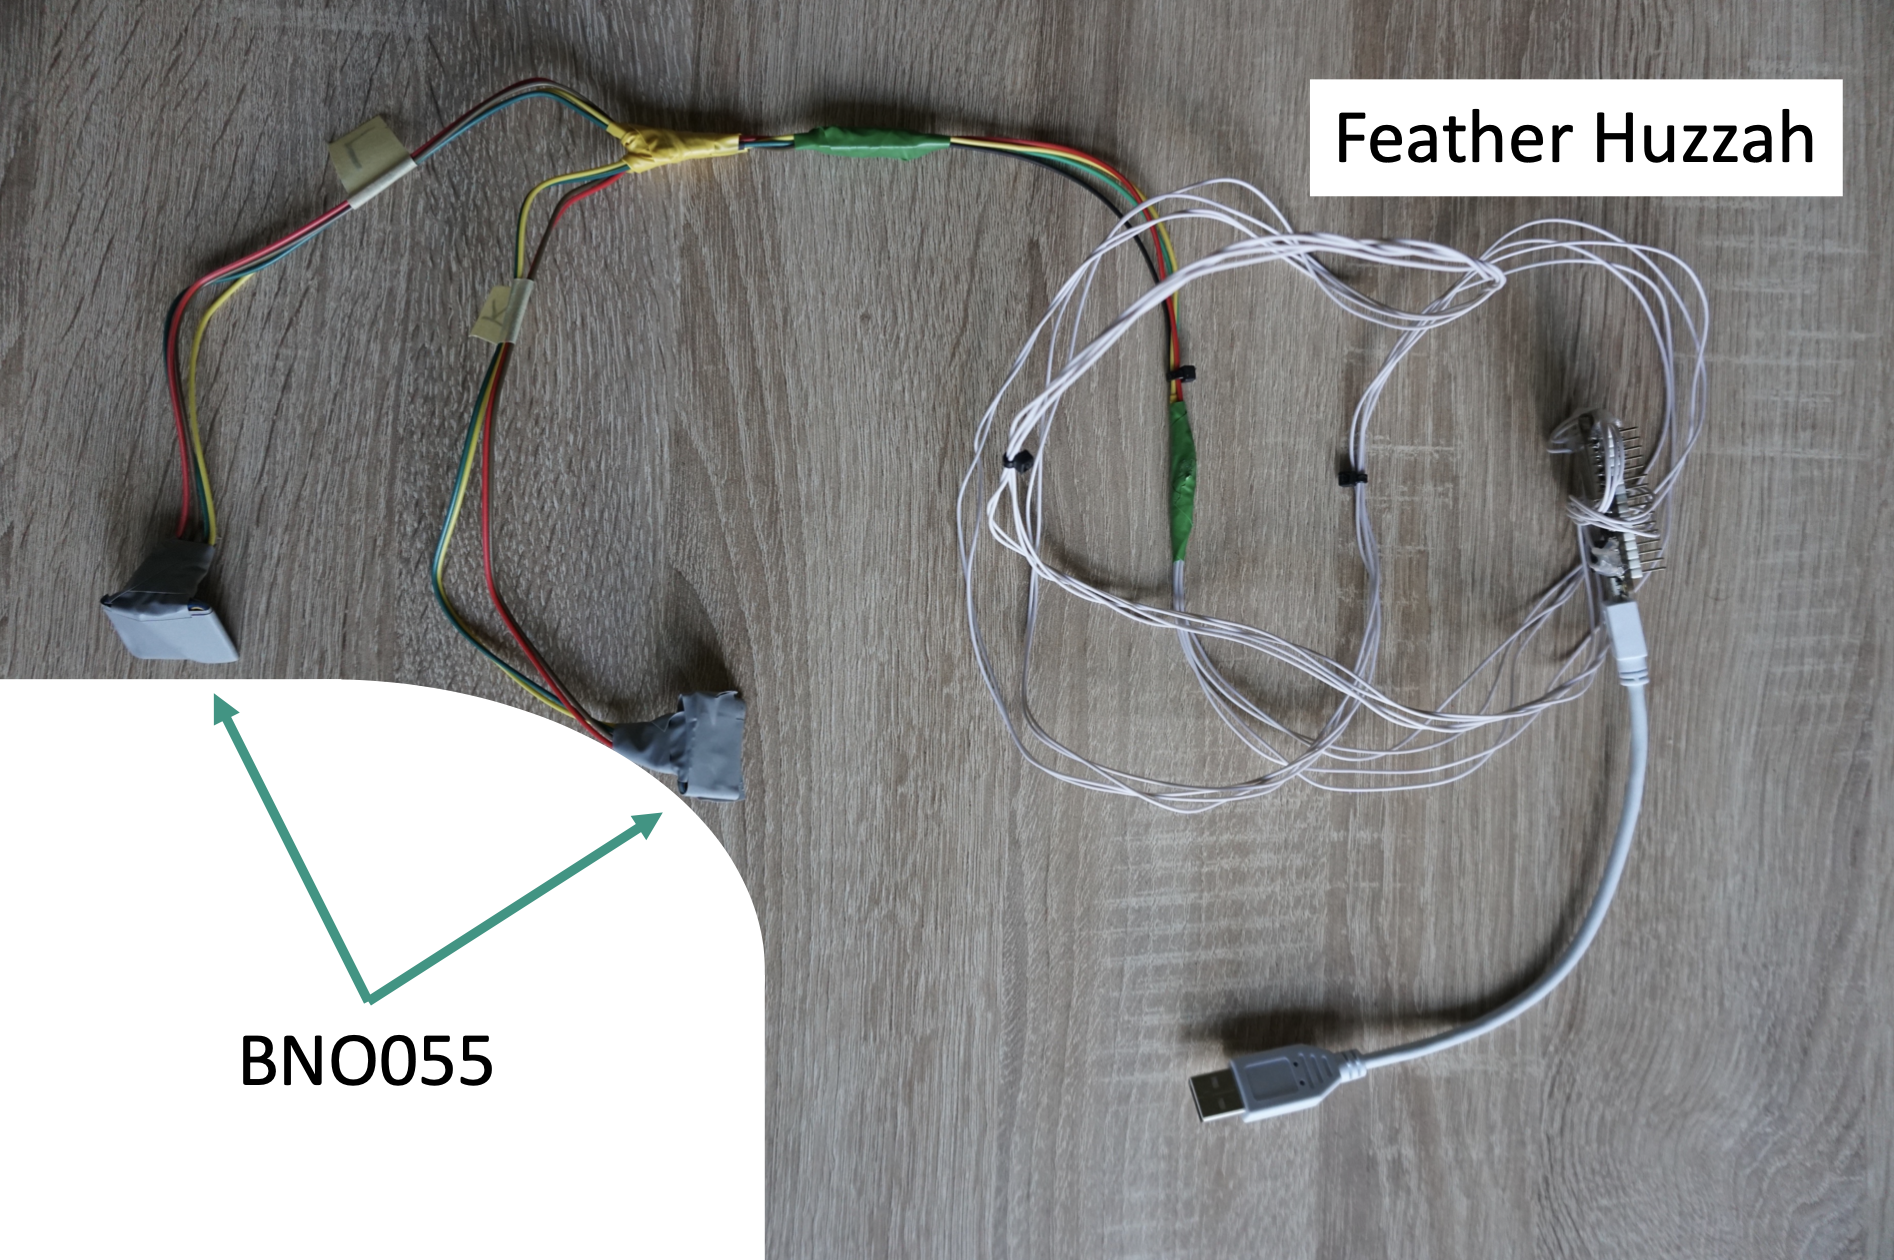
\includegraphics[width=0.5\textwidth]{src/media/hardware/real-bno.png}
\caption{Prototype of Arduino BNO055 with Feather Huzzah}
\label{image:real-bno}
\end{figure}

\subsubsection{Olimex EMG-Shield}
\label{subsub:emg}

\begin{figure}[h!]
\centering
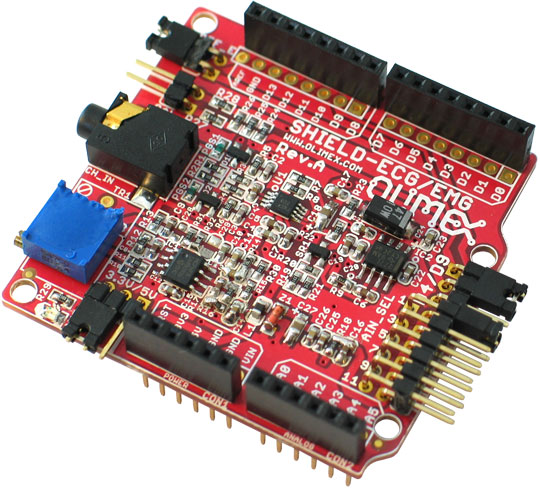
\includegraphics[width=0.5\textwidth]{src/media/hardware/emg.jpg}
\caption{Olimex EMG-Shield}
\label{image:emg}
\end{figure}

The EMG-Boards from Olimex can be stacked on top of each other, to allow readings from up to 6 channels at the same time. To capture the EMG signals from the left and right masseter muscles as well as from the left and right temporalis muscles, 4 EMG-Shields were used. The raw data from the board is analog, so an analog-to-digital (ADC) converter was needed, because the RPI doesn't have any analog input pins. For this purpose the Arduino Uno was used. The collected data was sent directly to the RPI over the Serial Protocol (USB).

\usedspecs{Serial}{256Hz}{EMG}{Olimex EMG-Shield in combination with Arduino Uno}{emg}

\begin{figure}[h!]
\centering
\includegraphics[width=0.5\textwidth]{src/media/hardware/real-emg-top.JPG}
\includegraphics[width=0.5\textwidth]{src/media/hardware/real-emg-side.JPG}
\caption{Prototype of EMG-Shields with Arduino Uno}
\label{image:real-emg}
\end{figure}


\section{Software}
\label{sec:software}
\chapter{Evaluation}
\label{ch:study}

The scope of the user study was to collect data from participants simulating bruxism as well as performing contrast jaw movements. All of the sensors but the throat microphone were recorded with the RPI. The throat microphone was connected directly to the laptop used to control the RPI.

A total of 10 participants, 1 female, were recruited, with the youngest participant aged 19 and the oldest aged 28. After inspecting the data, 4 recordings of the temporalis muscles were removed from the resulting dataset (3 recordings of the left temporalis muscle, 1 recording of the right temporalis muscle). In one of the cases, the EMG electrodes disconnected themselves during the study. In the other cases, the data was very noisy. 2 audio recordings were also discarded. The challenges during the data collection are discussed in ch. \ref{ch:sensor_attachment}. 

The experiment took about 30min. The collected usable data had a length of about 16min. Throughout the experiment, the participants were asked to stand still if not asked otherwise, especially in the phase with the bruxism-related tasks, and to focus their eyes on a circle on the wall in front of them. At every step, they were instructed by the experimenter about the exercise they had to perform and the moment they had to start and stop performing it. An overview of the user study can be seen in figure \ref{image:study_overview}.

\begin{figure}[h]
\centering
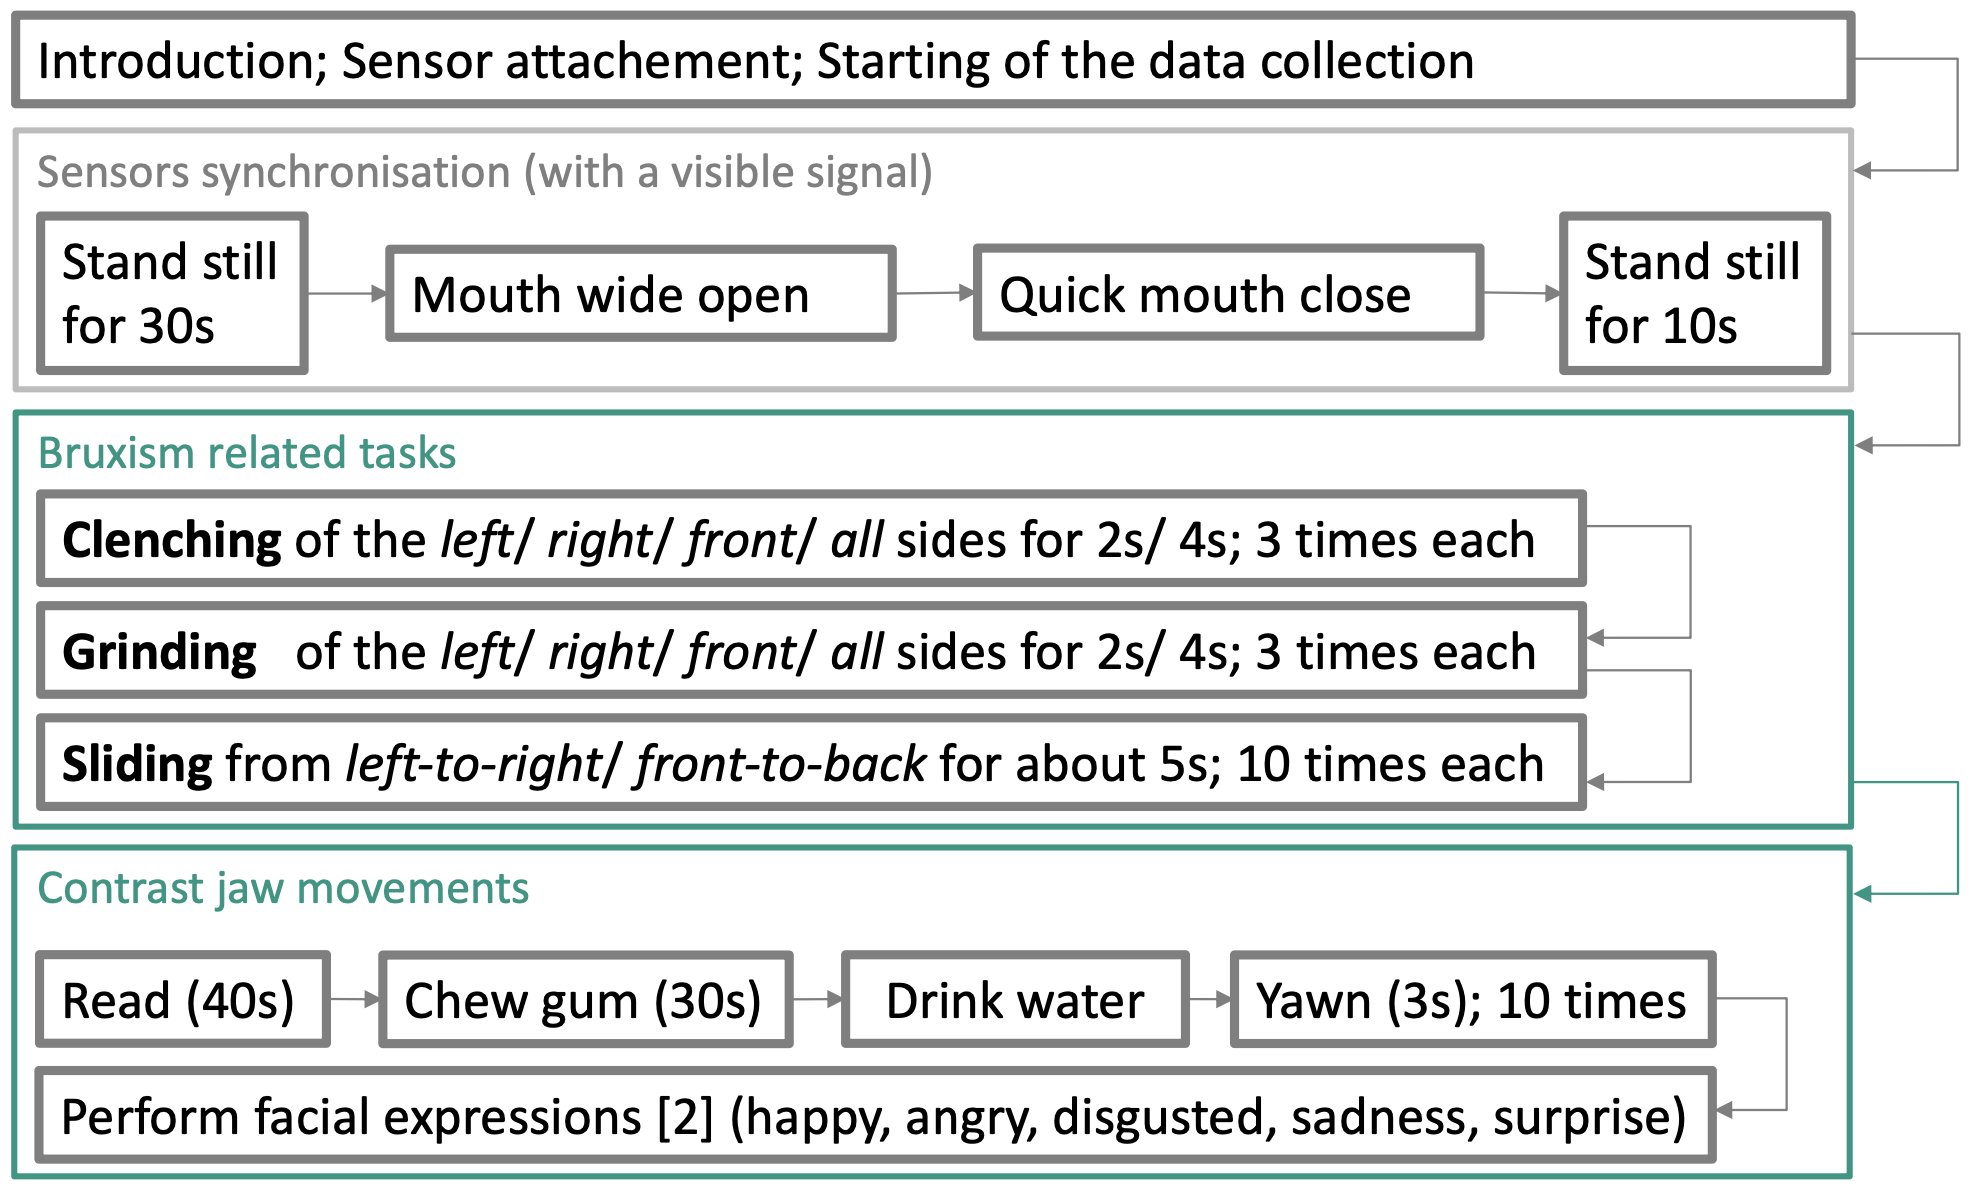
\includegraphics[width=0.8\textwidth]{src/media/study/study_overview.png}
\caption{User study overview}
\label{image:study_overview}
\end{figure}

\section{Data collection}

A total of 8 raw audio files were collected with the throat microphone. Six complete sets of time-series (a full set having N = 37 time-series) were used. In one set of time-series, the EMG recordings of the right temporalis muscle were corrupted (leaving n = 36 time-series). In the other three sets of time-series, the EMG recordings of the left temporalis muscle were corrupted (leaving n = 36 time-series for each set). The  study  yielded a total of 366 time-series collected with the RPI and eight audio recordings, with a total data removal of 1\% for the RPI (representing 10\% data removal of the collected EMG time-series) and 20\% for the audio recordings.

The time-series had a length of around 16min. The 37 time-series consists of the x, y, and z axis of the left (right) eSense earables gyroscope, x, y, and z axis of the left (right) eSense earables accelerometer, x, y, and z axis of the left (right) BNO055 gyroscope, x, y and z axis of the left (right) BNO055 accelerometer, w, x, y and z axis of the left (right) BNO055 quaternion, EMG signal for the left (right) masseter, left (right) temporalis, and GSR (table \ref{table:data_collection}).

\begin{table}[!h]
\centering
\begin{tabular}{|m{0.25\linewidth}|m{0.4\linewidth}|m{0.2\linewidth}|} 
 \hline
 Device & Time-series & Sample Rate \\ [0.5ex] 
 \hline\hline
 eSense earables &
        \begin{tabular}[t]{ll}
            Left gyroscope \texttt{x, y, z} \\
            Left accelerometer \texttt{x, y, z} \\
            \\
            Right gyroscope \texttt{x, y, z} \\
            Right accelerometer \texttt{x, y, z}
        \end{tabular} &
        \begin{tabular}[t]{ll}
            100Hz \\
            \\\\
            100Hz
        \end{tabular} \\
 \hline
 BNO055 &
        \begin{tabular}[t]{ll}
            Left gyroscope \texttt{x, y, z} \\
            Left accelerometer \texttt{x, y, z} \\
            Left quaternion \texttt{w, x, y, z} \\
            \\
            Right gyroscope \texttt{x, y, z} \\
            Right accelerometer \texttt{x, y, z} \\
            Right quaternion \texttt{w, x, y, z}
        \end{tabular} &
        \begin{tabular}[t]{ll}
            100Hz \\
            \\\\\\
            100Hz
        \end{tabular} \\
\hline
EMG &
        \begin{tabular}[t]{ll}
            Left masseter \\
            Right masseter \\
            Left temporalis \\
            Right temporalis
        \end{tabular} &
        \begin{tabular}[t]{ll}
            256Hz
        \end{tabular} \\
\hline
Throat Microphone &
        \begin{tabular}[t]{ll}
            Raw audio
        \end{tabular} &
        \begin{tabular}[t]{ll}
            44.1kHz
        \end{tabular} \\
\hline
GSR &
        \begin{tabular}[t]{ll}
            GSR
        \end{tabular} &
        \begin{tabular}[t]{ll}
            20Hz
        \end{tabular} \\
\hline
\hline
Total & 37 time-series \& 1 audio file & \\
\hline
\end{tabular}
\caption{Collected data overview}
\label{table:data_collection}
\end{table}


\section{Sensor Attachment}
\label{ch:sensor_attachment}

The sensor attachment was done as described in the table \ref{table:hardware_peripherals}. Some of the peripherals required special mounting based on the participants anatomy (see \ref{par:emg_attachment}) and some of the participants had trouble wearing some types of peripherals (see \ref{par:esense_attachment}, \ref{par:mic_attachment}).

\section{Study Design}

The participants were introduced to the user study and the concept of bruxism. After generating a pseudo-random code-name and acknowledging and accepting the terms of the data collection the sensors were attached and the data collection started.

\subsection{Sensor synchronization}
Even though the RPI already synchronizes the collected data from the connected sensors, using its internal clock, the throat microphone was connected to a separate device. To be able to align these time-series later, the participants were asked to perform a certain jaw movement, as a synchronization signal:
\begin{enumerate}
    \item Stand still for 30s;
    \item Mouth wide open;
    \item Quick mouth close;
    \item Stand still for 10s.
\end{enumerate}

\subsection{Bruxism related tasks}
In this phase the participants were asked to perform the following jaw movements to simulate bruxism:
\begin{itemize}
    \item \textbf{Clenching}: touch the requested sides with as much force as possible, without other jaw movements.
    \item \textbf{Grinding}: touch the requested sides with as much force as possible, with additional small jaw movements. Imagine that you are rubbing the touching teeth with one another;
    \item \textbf{Sliding}: move your lower jaw in the requested pattern.
\end{itemize}

The sequence of performing of these movements was repeated several times with different duration:
\begin{enumerate}
    \item Clench the \emph{left} side for \textbf{2s}, 3 times in total, with pauses in-between;
    \item Clench the \emph{right} side for \textbf{2s}, 3 times in total, with pauses in-between;
    \item Clench the \emph{front} side for \textbf{2s}, 3 times in total, with pauses in-between;
    \item Clench \emph{all sides} for \textbf{2s}, 3 times in total, with pauses in-between;
    \item pause for 5s.
    \item Clench the \emph{left} side for \textbf{4s}, 3 times in total, with pauses in-between;
    \item Clench the \emph{right} side for \textbf{4s}, 3 times in total, with pauses in-between;
    \item Clench the \emph{front} side for \textbf{4s}, 3 times in total, with pauses in-between;
    \item Clench \emph{all sides} for \textbf{4s}, 3 times in total, with pauses in-between;
\end{enumerate}

Similarly grinding was done next.

Then sliding was performed with the movement of the whole jaw:
\begin{enumerate}
    \item Slide from \emph{left-to-right} for about \textbf{5s}, 10 times in total;
    \item Slide from \emph{front-to-back} for about \textbf{5s}, 10 times in total;
\end{enumerate}

\subsection{Contrast jaw movements}
After the bruxism phase, it was important to record other typical jaw movements. For that following materials were prepared:
\begin{itemize}
    \item A text snippet (in both English and German language), with a time-to-read of about 40s;
    \item Chewing gum;
    \item A glass of water;
    \item 6 facial expressions from the KDEF \cite{lundqvist1998karolinska}, printed on paper.
\end{itemize}

The tasks were then done in the following order:
\begin{enumerate}
    \item Read the following text out loud, either in English or German;
    \item Chew a gum for \textbf{30s};
    \item Drink a glass of water;
    \item Yawn for about \textbf{3s} or longer if you feel so, 10 times in total;
    \item Perform the following facial expression as you see it for about \textbf{4s}, relax your face, and proceed with the next facial expression, 12 times in total.
\end{enumerate}

After that, the data collection was stopped. The raw audio data was saved on the laptop and the generated \texttt{.csv} files were copied from the RPI to the laptop using \texttt{scp}. The whole user study duration was about 35min.


\section{Survey}

Each participant completed a survey at the end of the user study. This included demographic questions and questions about the wear and feel of the peripherals. The results are presented in the table \ref{table:masseter_asymmetry}, \ref{table:devices_comfort} and \ref{table:devices_score}. It appears that the participants found the BNO055s the most comfortable.

\begin{table}[!h]
\centering
\begin{tabular}{|>{\raggedright}m{0.4\linewidth}||m{0.11\linewidth}|m{0.11\linewidth}|m{0.11\linewidth}|m{0.11\linewidth}|} 
 \hline
  & Std. dev. & Var. & Min & Max \\ [0.5ex] 
 \hline\hline
 Visible difference between masseter muscles & 1.12 & 1.06 & -2 & 2 \\
 \hline
\end{tabular}
\caption{Masseter muscle asymmetry (-2 = left side is bigger, 2 = right side is bigger)}
\label{table:masseter_asymmetry}
\end{table}

\begin{table}[!h]
\centering
\begin{tabular}{|>{\raggedright}m{0.4\linewidth}||m{0.11\linewidth}|m{0.11\linewidth}|m{0.11\linewidth}|m{0.11\linewidth}|} 
 \hline
  & Std. dev. & Var. & Min & Max \\ [0.5ex] 
 \hline\hline
 Throat microphone & 1.07 & 1.03 & 0 & 3 \\
 \hline
 eSense earables & 0.77 & 0.88 & 0 & 3 \\
 \hline
 EMG electrodes & 0.28 & 0.53 & 2 & 3 \\
 \hline
 BNO055 & 0.28 & 0.53 & 2 & 3 \\
 \hline
\end{tabular}
\caption{Participants opinion on the devices comfort (0 = very uncomfortable, 3 = very comfortable).}
\label{table:devices_comfort}
\end{table}

\begin{table}[!h]
\centering
\begin{tabular}{|>{\raggedright}m{0.4\linewidth}||m{0.11\linewidth}|m{0.11\linewidth}|m{0.11\linewidth}|m{0.11\linewidth}|} 
 \hline
  Device & Std. dev. & Var. & Min & Max \\ [0.5ex] 
 \hline\hline
 Throat microphone & 0.12 & 0.02 & 0.70 & 0.97 \\
 \hline
 eSense earables & 0.10 & 0.01 & 0.71 & 1 \\
 \hline
 EMG electrodes & 0.17 & 0.03 & 0.43 & 1 \\
 \hline
 BNO055 & 0.10 & 0.01 & 0.75 & 1 \\
 \hline
\end{tabular}
\caption{Device score based on participants' answers on overall wear and feel (0 = lowest score, 1 = highest score).}
\label{table:devices_score}
\end{table}

\section{Analysis}
\label{ch:methodology}

\subsection{Labeling}

\paragraph{Data irregularity}

The sensors are set to deliver data at a predefined sample rate. But in practice, this value fluctuates somewhat. As a result, the datapoints of the collected time-series are not aligned. Even the data of a single time-series may be captured at different intervals while maintaining the designed sample rate. In such cases, the data we deal with is \emph{irregular} (e.g. \ref{image:irregular-data}).

To remove the irregularity from the data and make it \emph{regular}, the time-series can be resampled (e.g. \ref{image:regular-data}). At this moment, we can choose the resampling rate equal to the original sampling rate (i.e., aligning the datapoints of a time-series to fixed intervals) or select a higher or lower sample rate. As we don't require high-precision timestamps in the nanoseconds range, it is enough to have precision in the tens or hundreds of milliseconds. After some trials, the datasets were resampled to 20Hz. The missing values were linearly interpolated.

\begin{figure}[!h]
\centering
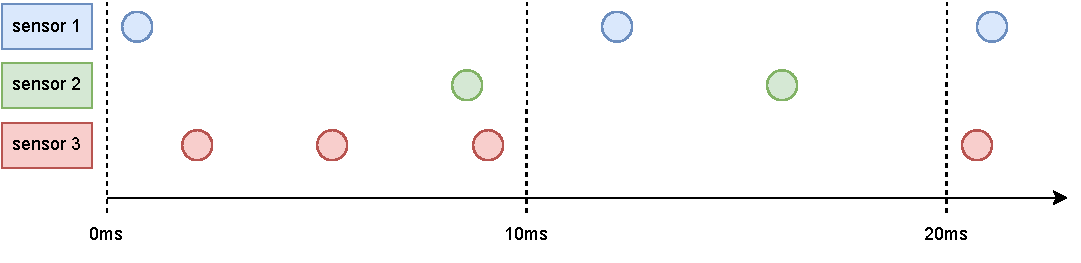
\includegraphics[width=\textwidth]{src/media/methodology/irregular-data2.pdf}
\caption{Example of irregular data. Circles represent the moment a payload was captured. Colors relate the point in time to the sensor of origin}.
\label{image:irregular-data}
\end{figure}

\begin{figure}[!h]
\centering
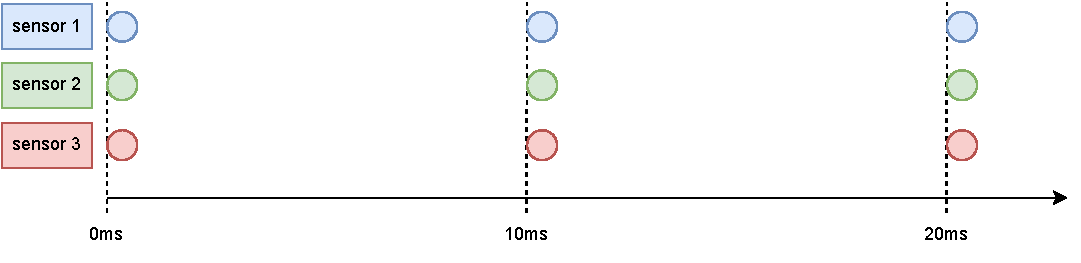
\includegraphics[width=\textwidth]{src/media/methodology/regular-data.pdf}
\caption{Example of regular data. Circles represent the moment a payload was captured. Colors relate the point in time to the sensor of origin}.
\label{image:regular-data}
\end{figure}

\paragraph{Label methodology}

The labeling was done manually after the user study concluded. To ease this process, the following procedure was done:

\begin{enumerate}
    \item For each dataset, the maximum of the minimum timestamps was calculated (i.e., the first timestamp of the last sensor that started delivering data). Then all timestamps in a dataset were offset by the calculated timestamp. As a result, if plotted, having the time on the X-axis, the time-series will start at 0.
    \item The values for each time-series were z-normalized, and the plots were presented overlapping in a single figure (one of such datasets is shown in fig. \ref{image:dataset_overview}).
\end{enumerate}

To z-normalize the values for each time-series the following formula was used:

\[ y := \frac{y - \mu}{\sigma} \]

where $y$ is a value in the time-series, $\mu$ is the mean, and $\sigma$ is the standard deviation. 

The data aligned perfectly, and different activity types performed during the user study can be precisely located.

\paragraph{Label types}

All the time ranges with the bruxism-related tasks were labeled as 1 (i.e., is bruxism). The rest of the datapoints else was labeled as 0 (i.e., no bruxism).

\paragraph{Window selection}

A sliding window approach was applied, which is the standard procedure in time-series data processing. The sliding window had a length of 1.6s with 50\% overlap (0.8s). This ensures that we are grouping enough data points together and not missing transitions between muscle contractions or contraction bursts. The window was labeled by the dominant event in that window; If the larger portion of the window contains bruxism data and a smaller portion of silent data, the window would be labeled as bruxism. If the split is equal, then the window is labeled as silent \cite{bondareva2021earables}.

This resulted in windows having 32 datapoints for each of the 37 time-series, yielding 1184 features.

\subsection{Classification}

The classification was done by using a brute-force approach. Four traditional machine learning classifiers from sklearn were trained: random forest (RF), k-nearest neighbors (kNN), support vector machine (SVM), and decision tree (DT).

\paragraph{Brute-force Approach Overview}

The time-series were generalized into the following groups:

\begin{listing}[!h]
\begin{minted}
[
frame=lines,
framesep=2mm,
baselinestretch=1.2,
fontsize=\footnotesize,
linenos,
breaklines
]
{python}
timeseries_groups = {
    "bno_gyro": ['x28_gyro_x', 'x28_gyro_y', 'x28_gyro_z', "x29_gyro_x", "x29_gyro_y", "x29_gyro_z"],
    "bno_acc": ["x28_acceleration_x", "x28_acceleration_y", "x28_acceleration_z", "x29_acceleration_x", "x29_acceleration_y", "x29_acceleration_z"],
    "bno_quat": ["x28_quaternion_w", "x28_quaternion_x", "x28_quaternion_y", "x28_quaternion_z", "x29_quaternion_w", "x29_quaternion_x", "x29_quaternion_y", "x29_quaternion_z"],

    "ble_gyro": ["gyro_x", "gyro_y", "gyro_z", "gyro_x_2", "gyro_y_2", "gyro_z_2"],
    "ble_acc": ["acceleration_x", "acceleration_y", "acceleration_z", "acceleration_x_2", "acceleration_y_2", "acceleration_z_2"],

    "gsr": ["gsr"],

    "masseter": ["masseter_left", "masseter_right"],

    "temporalis": ["temporalis_left", "temporalis_right"]
}
\end{minted}
\caption{Dataset time-series abstractions}
\label{listing:dataset_abstractions}
\end{listing}

then a power set (excluding the empty set) was computed for the set of the groups of time-series: \texttt{"bno\_gyro", "bno\_acc", "bno\_quat", "ble\_gyro", "ble\_acc", "gsr", "masseter", "temporalis"} (8 in total). For every two-sided sensor, both sides were placed in the same group. Bruxers tend to have one side of the masticatory muscles overdeveloped, which will lead to cleaner data samplings and better results. But this is highly individual, and to cover every possible use-case scenario, the data from both sides is needed.

The resulted power set had a length of 255 (\(2^8 - 1\))

For Every such group, an array of windows with the corresponding time-series from every dataset was computed. The window labels from every dataset were stored in an array as well so that a window will share the same positional index in the array as its label does.

\paragraph{Brute-force training}

Every feature set (group of time-series) windows were split in 20:80 ratio (20 for testing, 80 for training) and passed sequentially to a model classifier.

\paragraph{Brute-force evaluation}

For every model---feature-set pair, an accuracy score was calculated.

\chapter{Results}

\section{Overview}

The top performing models---feature-set pair was RF (\texttt{"bno\_gyro", "bno\_quat", "ble\_acc", "masseter", "temporalis"}) with a score of \texttt{0.915}.

Table \ref{table:top_5_per_group} depicts the top 5 best performing models sorted by the feature-set size. It was sorted this way because, alongside the theoretical highest score, it is also important that the feature-set has a practical application in real life. As an example RF (\texttt{"bno\_quat"}) (score = 0.881) will be valued higher ten the RF (\texttt{"bno\_gyro", "bno\_quat", "ble\_acc", "masseter", "temporalis"}) (score = 0.915). It's mainly because it's much easier to design a less error-prone prototype using just one type of sensor. Also, it is a much more practical and non-invasive solution for the end-user to wear.

Clearly, RF outperforms other classifiers by far. But the most considerable insight here is that the \texttt{bno\_quat} appears in every top for every feature-set size. It gives two main takeaways:
\begin{itemize}
    \item The sensor fusion (the process of calculating the quaternion using the 9 DOF data provided by the IMU) of the BNO055 helps to increase the IMU accuracy for bruxism detection;
    \item A fine-tuned EMG may ultimately be the ground truth in bruxism assessment (achieving 100\% accuracy \cite{Sonmezocak2021}). Still, a pair of IMUs remains cheaper and more practical, and this study also showed a good enough option for bruxism detection.
\end{itemize}

\begin{table}[h!]
\begin{tabular}{lrr}
\toprule
                                                 Model, feature-set pair &  Score &  Feature-set size \\
\midrule
                                                           RF (bno\_quat) &  0.881 &                 1 \\
                                                          kNN (bno\_quat) &  0.880 &                 1 \\
                                                           DT (bno\_quat) &  0.849 &                 1 \\
                                                            RF (ble\_acc) &  0.846 &                 1 \\
                                                            RF (bno\_acc) &  0.844 &                 1 \\
                                                RF (bno\_quat,temporalis) &  0.904 &                 2 \\
                                                  RF (bno\_quat,ble\_gyro) &  0.896 &                 2 \\
                                                  RF (bno\_gyro,bno\_quat) &  0.890 &                 2 \\
                                                  kNN (bno\_quat,ble\_acc) &  0.888 &                 2 \\
                                                       RF (bno\_quat,gsr) &  0.887 &                 2 \\
                                       RF (bno\_quat,ble\_gyro,temporalis) &  0.906 &                 3 \\
                                          RF (bno\_gyro,bno\_acc,bno\_quat) &  0.904 &                 3 \\
                                              RF (bno\_gyro,bno\_quat,gsr) &  0.897 &                 3 \\
                                           RF (bno\_acc,bno\_quat,ble\_acc) &  0.894 &                 3 \\
                                         RF (bno\_gyro,bno\_quat,masseter) &  0.894 &                 3 \\
                               RF (bno\_gyro,bno\_quat,ble\_acc,temporalis) &  0.907 &                 4 \\
                                   RF (bno\_quat,ble\_gyro,gsr,temporalis) &  0.906 &                 4 \\
                                RF (bno\_gyro,bno\_acc,ble\_acc,temporalis) &  0.905 &                 4 \\
                                   RF (bno\_gyro,bno\_quat,gsr,temporalis) &  0.905 &                 4 \\
                              RF (bno\_gyro,bno\_quat,ble\_gyro,temporalis) &  0.903 &                 4 \\
                      RF (bno\_gyro,bno\_quat,ble\_acc,masseter,temporalis) &  0.915 &                 5 \\
                            RF (bno\_acc,bno\_quat,ble\_acc,gsr,temporalis) &  0.913 &                 5 \\
                     RF (bno\_gyro,bno\_quat,ble\_gyro,masseter,temporalis) &  0.913 &                 5 \\
                      RF (bno\_gyro,bno\_acc,bno\_quat,masseter,temporalis) &  0.910 &                 5 \\
                       RF (bno\_gyro,bno\_acc,bno\_quat,ble\_acc,temporalis) &  0.909 &                 5 \\
             RF (bno\_gyro,bno\_acc,bno\_quat,ble\_gyro,masseter,temporalis) &  0.915 &                 6 \\
                  RF (bno\_gyro,bno\_acc,bno\_quat,ble\_gyro,gsr,temporalis) &  0.913 &                 6 \\
              RF (bno\_gyro,bno\_acc,bno\_quat,ble\_gyro,ble\_acc,temporalis) &  0.911 &                 6 \\
                  RF (bno\_gyro,bno\_quat,ble\_acc,gsr,masseter,temporalis) &  0.910 &                 6 \\
                  RF (bno\_gyro,bno\_quat,ble\_gyro,ble\_acc,gsr,temporalis) &  0.905 &                 6 \\
          RF (bno\_acc,bno\_quat,ble\_gyro,ble\_acc,\\gsr,masseter,temporalis) &  0.913 &                 7 \\
     RF (bno\_gyro,bno\_acc,bno\_quat,ble\_gyro,\\ble\_acc,masseter,temporalis) &  0.906 &                 7 \\
          RF (bno\_gyro,bno\_acc,bno\_quat,ble\_gyro,\\ble\_acc,gsr,temporalis) &  0.902 &                 7 \\
            RF (bno\_gyro,bno\_acc,bno\_quat,ble\_gyro,\\ble\_acc,gsr,masseter) &  0.900 &                 7 \\
         RF (bno\_gyro,bno\_acc,bno\_quat,ble\_gyro,\\gsr,masseter,temporalis) &  0.900 &                 7 \\
 RF (bno\_gyro,bno\_acc,bno\_quat,ble\_gyro,ble\_acc,\\gsr,masseter,temporalis) &  0.901 &                 8 \\
 DT (bno\_gyro,bno\_acc,bno\_quat,ble\_gyro,ble\_acc,\\gsr,masseter,temporalis) &  0.852 &                 8 \\
kNN (bno\_gyro,bno\_acc,bno\_quat,ble\_gyro,ble\_acc,\\gsr,masseter,temporalis) &  0.701 &                 8 \\
SVM (bno\_gyro,bno\_acc,bno\_quat,ble\_gyro,ble\_acc,\\gsr,masseter,temporalis) &  0.670 &                 8 \\
\bottomrule
\end{tabular}


\caption{Model, feature-sets pairs with score. Only top 5 values are shown for each feature-set size}.
\label{table:top_5_per_group}
\end{table}

\section{Data Quality}

\paragraph{eSense earables \& BNO055}

The IMU time-series were generally clean and didn't present any challenge or corruption (e.g. \ref{plot:ble_right_gyro_grind}).

\paragraph{EMG}

The EMG quality signal is very dependent on the placement of the electrodes. It can produce precise and indistinguishable patterns (e.g., fig. \ref{plot:masseter_right_clenching}, \ref{plot:masseter_left_clenching}, \ref{plot:temporalis_right}, \ref{plot:masseter_reading}). Otherwise, if the electrodes were misplaced even by 1mm, the time-series had to be discarded, as nothing other than noise was recorded (e.g. fig. \ref{plot:temporalis_left}).

\paragraph{Throat Microphone}

The throat microphone performed poorly, and it wasn't able to catch the vibrations from the bruxism. The audio files were not used later in the classification.

\paragraph{GSR}

The collected data showed a similar pattern among all participants: Higher values in the bruxism simulation phase, followed by an immediate decay during the contrast jaw movements phase (fig. \ref{plot:gsr}).

\include{tex/chapter/results}
\chapter{Conclusions}
\label{ch:conslucions}

\section{Summary}

A brute-force approach was used to classify bruxism-related events. Four traditional classifiers were combined with different recorded time-series sets. Quaternion data from the IMUs placed on the back sides of the jaw with the random forest classifier yielded the best performance score with the least amount of sensors. It achieved 88\% accuracy. The best performing score overall was 91.5\% achieved by the random forest classifier with the BNO055 gyroscope and quaternion, eSense earables accelerometer, masseter, and temporalis time-series (from both sides each). As the IMUs tend to be cheaper than the EMG and are already present in various wearables (e.g. eSense earables) it once more confirms their potential in bruxism detection.

This study summarizes the use of 5 different devices with the scope of classifying bruxism-related events. The COVID-19 Pandemic may have also started another wave of a bruxism pandemic. The overall increase in the stress level may as well increase the prevalence of awake bruxism. A cheap and practical device is needed, that will have the ability to diagnose potential patients before it will lead to discomfort or teeth damage. The device selection was done based on previous research in the field and then combined together in a custom-built prototype. While selecting the devices we tried to maximize the use of the \emph{potential area} on the human head and neck, where a bruxism-induced signal may be recorded. A user study was designed to include bruxism-related jaw movements (clenching, grinding, and sliding) and contrasting \emph{regular} jaw movements (talking, drinking, chewing, smiling, etc.). All of the selected devices for the prototype were used at the same time during every user study.

\section{Limitations \& Future Work}

The study was done in a controlled environment, and the presented results may only be compared only in the context of this study. It is important to mention, that the custom-built prototype was just used as a framework to generate a reference.

The results of this study show that the sensor fusion of the IMU data appears the most promising feature to have a wearable device in the vicinity of the jaw. The closer to the jaw, the better the accuracy.

Bruxism happens mostly unconsciously. Prolonged periods appear during a patient's sleep. An EMG-oriented device may actually be a better choice for a sleep use case. A comparison with a much more mature device with IMUs is needed to be done in-the-wild.

Alternative ways of labeling and data segmentation can be explored. In an in-the-wild environment, bigger duration trends can be tracked. The performance in such cases should ideally correlate with the lessening of the bruxism occurrence over time.

More advanced machine learning approaches for time-series classification may also be useful.

The labeling of the data was in itself a very cumbersome and error-prone process. As we had to rely on visual clues in the time-series, as well as on timing (estimated duration of performed tasks and the duration of the pauses in-between). The keyboard event listener coroutine (see ch. \ref{ch:Implementation}) can be improved and extended to create the labels during the runtime. Either the experimenter or the participant itself can press (or hold) a button, to indicate a start or end of an action. This coroutine can be completely extracted from the framework and used as a separate device or as a software module.

\section{Challenges}
\label{sub:attachment_problems}

\subsection{eSense earables}
\label{par:esense_attachment}

Because of the design of the earables to be placed in the ear, some of the participants had trouble fitting them inside of their ears. Because the audio playback or audio recording with the built-in microphone was out of the scope of this study, the earables were secured with skin-friendly tape.

\subsection{EMG-Electrodes}
\label{par:emg_attachment}

To collect EMG signals, special electrodes must be placed on the skin surface covering the target muscle. It is not a trivial task, as the anatomy of the participant dictates the optimal spot of the electrode placement. The following research paper was used as a reference to find the optimal EMG spots \cite{sabaneeff2017proposal}.

\begin{figure}[h!]
\centering
 \begin{subfigure}[b]{0.49\textwidth}
    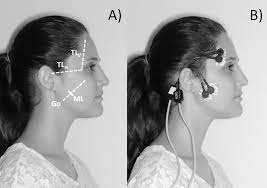
\includegraphics[width=\textwidth]{src/media/study/emg1.jpeg}
    \caption{ (A) Reference lines drawn on the face of a volunteer;
(B) electrodes positioned over the AT and SM muscles. \cite{sabaneeff2017proposal}}
  \end{subfigure}
 \hfill
 \begin{subfigure}[b]{0.49\textwidth}
    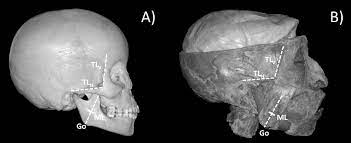
\includegraphics[width=\textwidth]{src/media/study/emg2.jpeg}
    \caption{ (A) The lateral view of the skull shows the reference lines used
in this study: TLV, TLH, and ML. The small thick line represents an
intersection at 40\% the length of ML from Go landmark; (B) Lateral
view of deep facial planes, evidencing the AT and SM muscles and their
relationship with anatomical landmarks and reference lines adopted. \cite{sabaneeff2017proposal}}
  \end{subfigure}
\caption{Optimal EMG spots for masticatory muscles by \cite{sabaneeff2017proposal}}
\label{image:real-emg}
\end{figure}

The following EMG electrode fig. \ref{image:emg_electrode} was used. For every target muscle, a pair of such electrodes is needed. Additionally, a reference electrode must be also placed on a neutral part of the head. The reference cables were fused together and connected to an electrode placed under the participant's chin.

The masticatory muscles are relatively small, so a slice of the adhesive foam was removed to bring the conductive parts of the two electrodes placed on one muscle, closer together. Even with this modification, the temporalis muscle was hard to capture, as even a misplace of 1mm from the optimal spot will introduce noise, or will capture the EMG signal of the nearby muscles (i.e. orbicularis muscle responsible for blinking).

\begin{figure}[h]
\centering
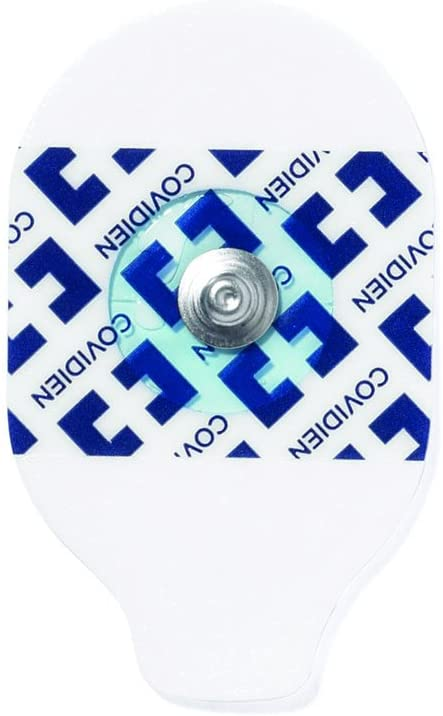
\includegraphics[width=0.2\textwidth]{src/media/study/electrode.jpg}
\caption{EMG electrode (57 x 34mm)}
\label{image:emg_electrode}
\end{figure}

\subsection{Throat Microphone}
\label{par:mic_attachment}

The throat microphone used in this study didn't have any adjustment possibilities. 2 of the participants had a smaller neck circumference, and as a result, it was not possible to capture the eventual vibrations that would propagate through the neck.


\include{tex/chapter/future_work}
% \chapter{Summary}
\label{ch:Summary}


\chapter{Code Availability}
The complete code for the custom-built framework can be found under \url{https://github.com/trupus/bruxism-benchmark}

%% ----------------
%% |   Appendix   |
%% ----------------

\appendix
\chapter{Plots}
% \chapter*{Appendix}
\begin{sidewaysfigure}[h]
\centering
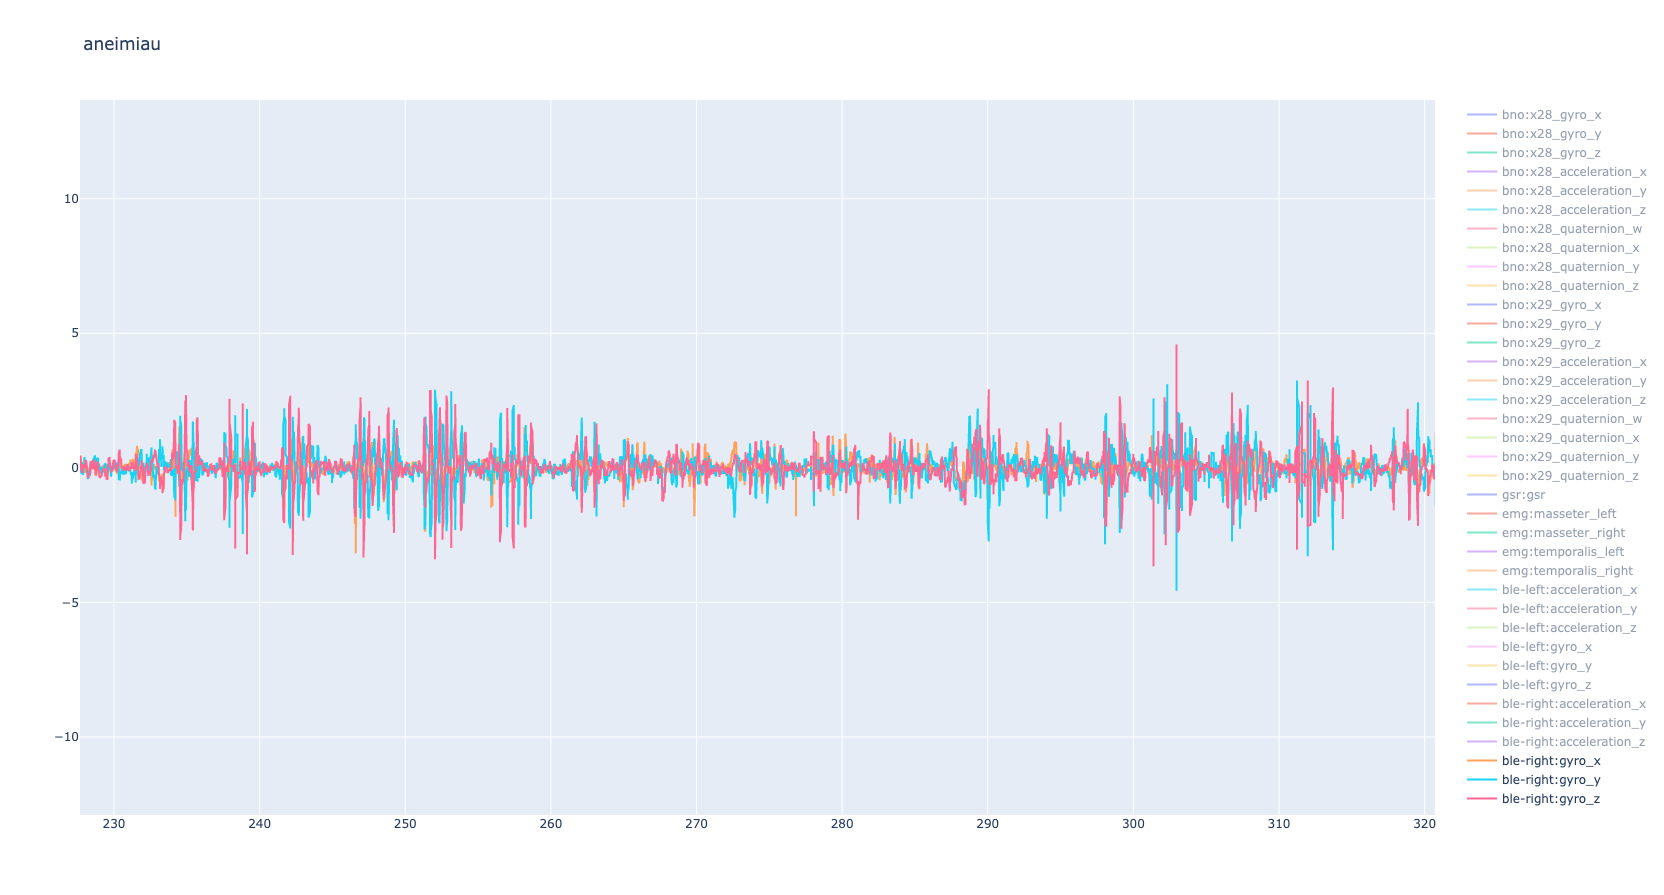
\includegraphics[width=\textwidth]{src/media/study/plots/ble_right_gyro_grind.png}
\caption{Example of a right eSense earable gyroscope x, y, and z time-series slice. The x, y, and z plots are overlapped. From left to right: 3x2s grinding with the right side; 3x4s grinding with the right side; 3x2s grinding with the front side; 3x4s grinding with the front side; 3x2s grinding with all sides; 3x4s grinding with all sides}
\label{plot:ble_right_gyro_grind}
\end{sidewaysfigure}

\begin{sidewaysfigure}[h]
\centering
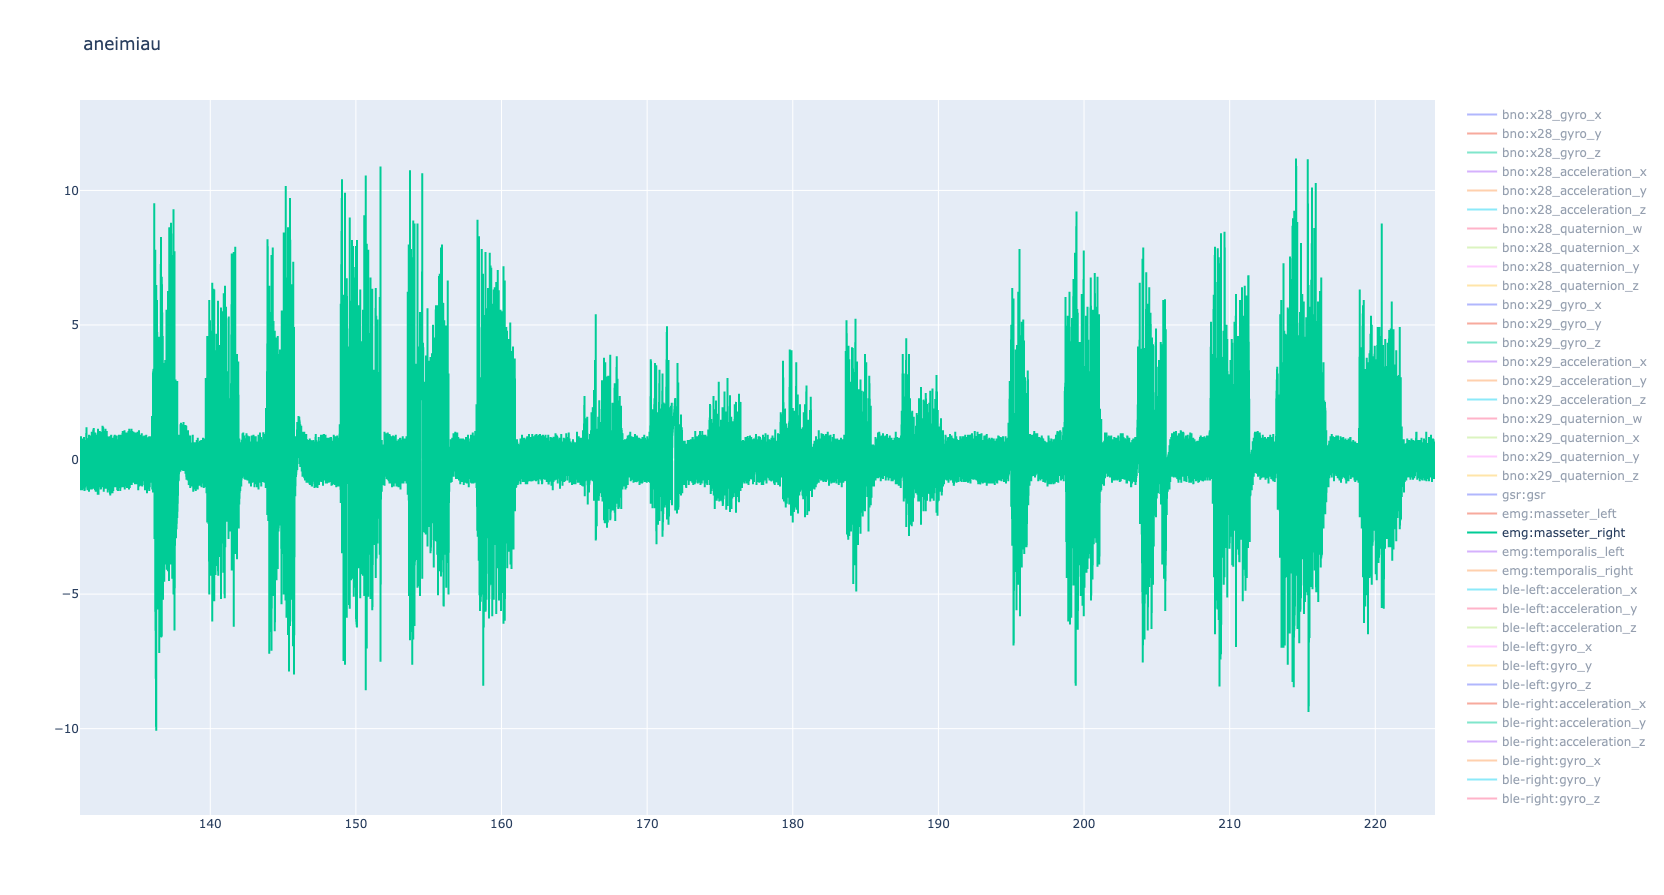
\includegraphics[width=\textwidth]{src/media/study/plots/masseter_right_clenching.png}
\caption{Example of a right masseter time-series slice. From left to right: 3x2s clenching with the right side; 3x4s clenching with the right side; 3x2s clenching with the front side; 3x4s clenching with the front side; 3x2s clenching with all sides; 3x4s clenching with all sides}
\label{plot:masseter_right_clenching}
\end{sidewaysfigure}

\begin{sidewaysfigure}[h]
\centering
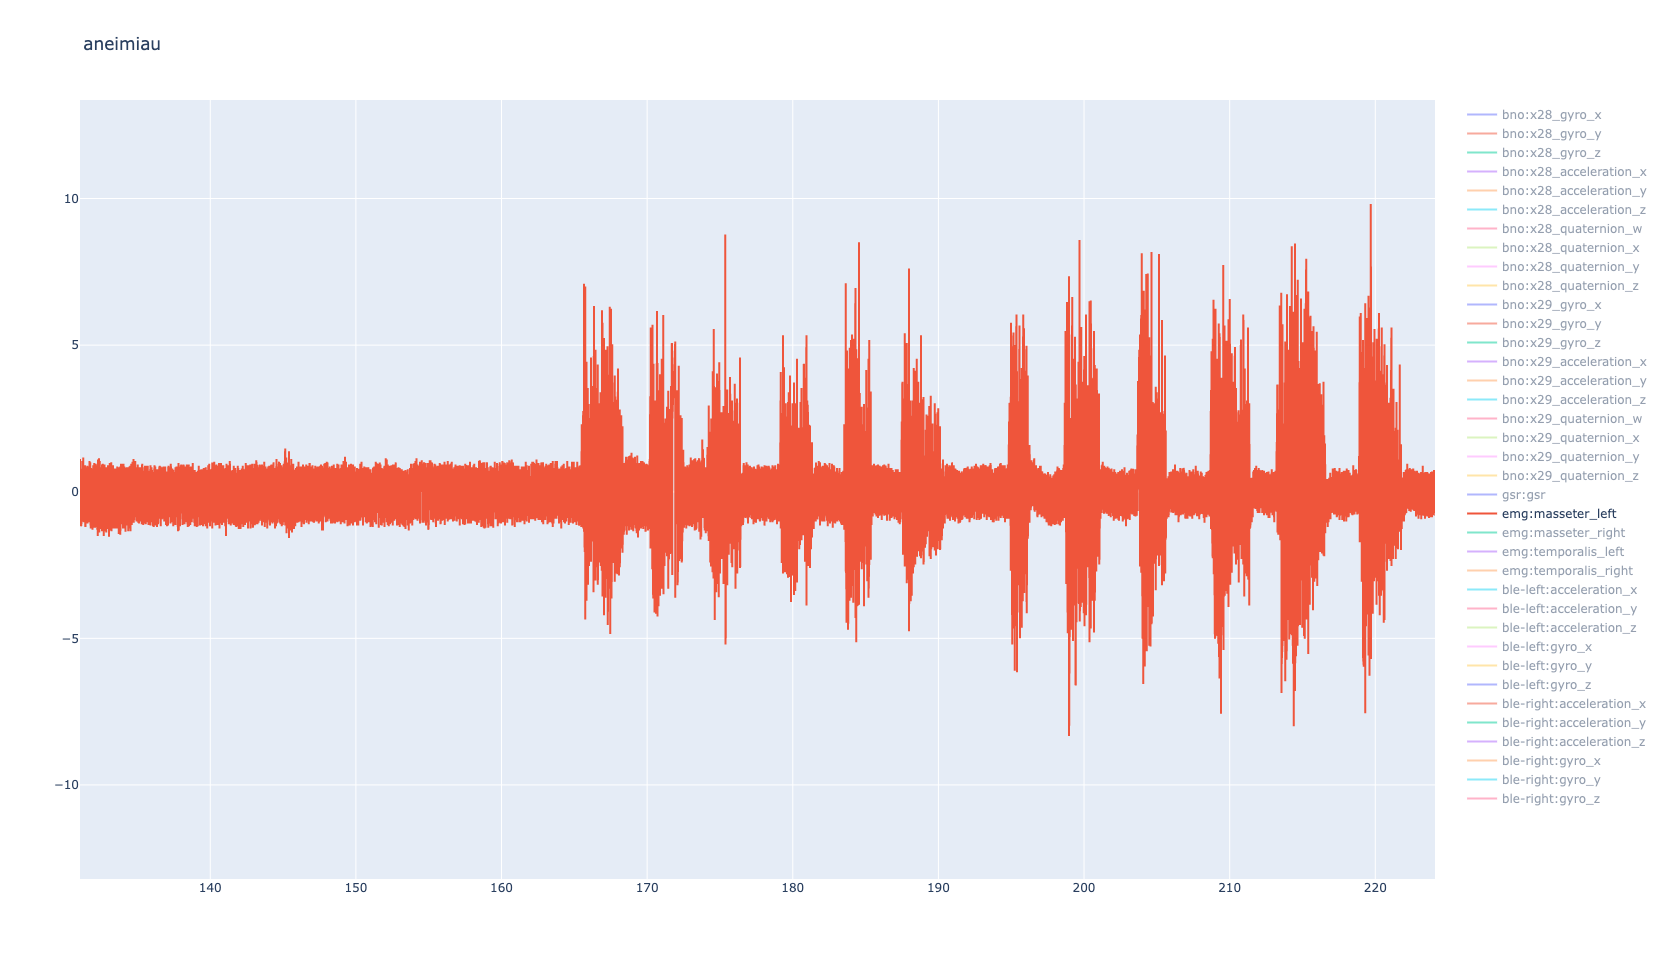
\includegraphics[width=\textwidth]{src/media/study/plots/masseter_left_clenching.png}
\caption{Example of a left masseter time-series slice. From left to right: 3x2s clenching with the right side; 3x4s clenching with the right side; 3x2s clenching with the front side; 3x4s clenching with the front side; 3x2s clenching with all sides; 3x4s clenching with all sides}
\label{plot:masseter_left_clenching}
\end{sidewaysfigure}

\begin{sidewaysfigure}[h]
\centering
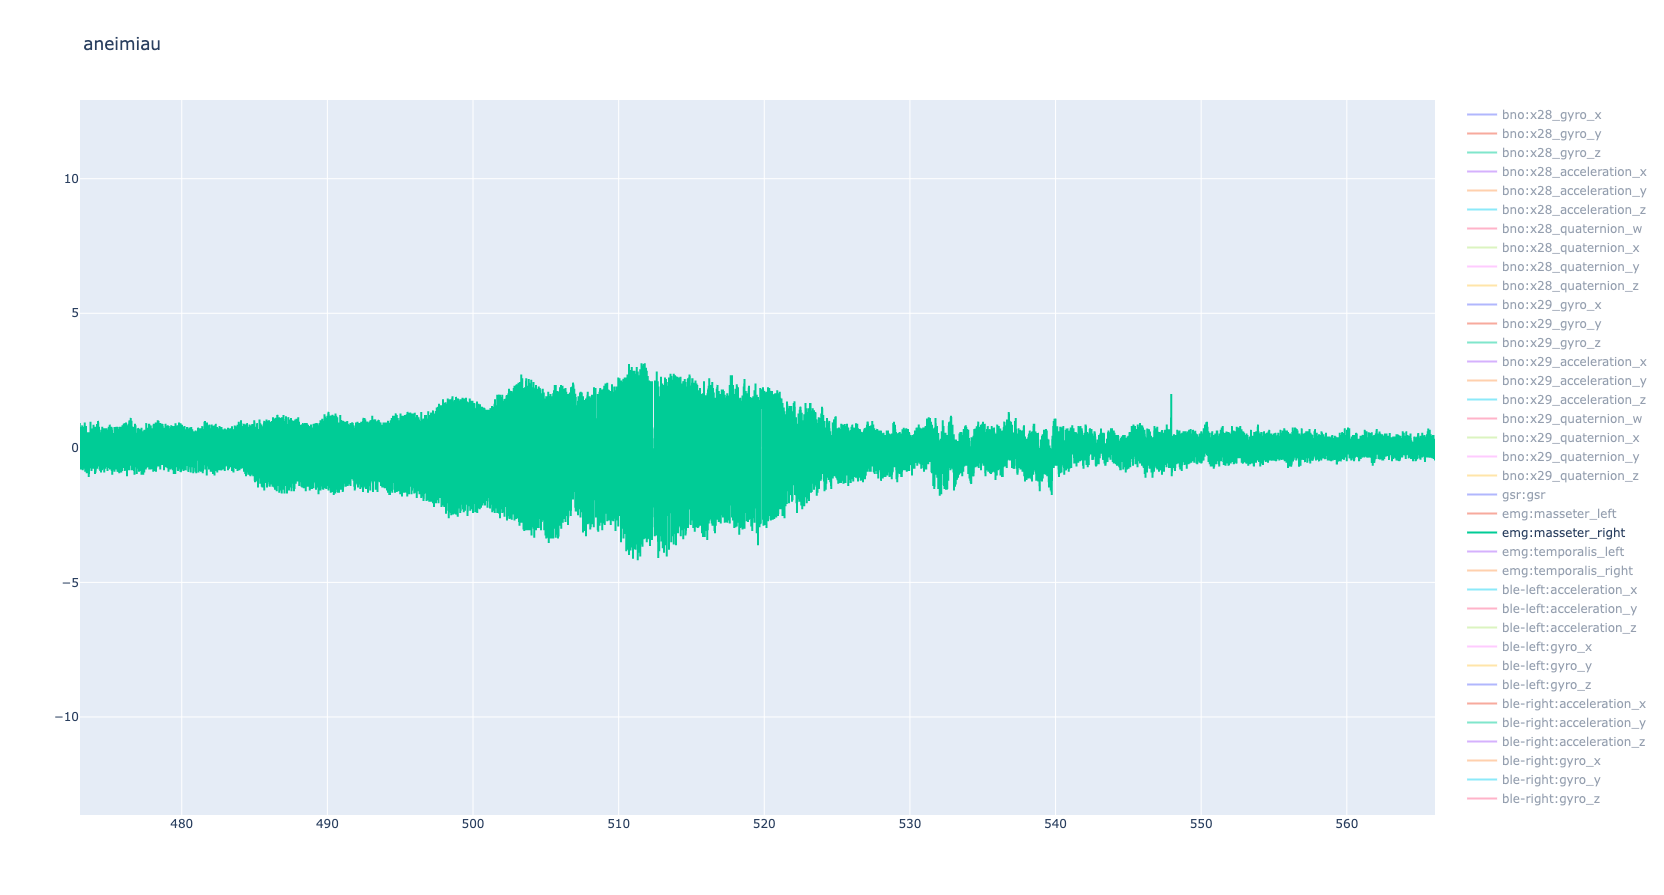
\includegraphics[width=\textwidth]{src/media/study/plots/masseter_right_talking.png}
\caption{Example of a right masseter time-series slice. Reading}
\label{plot:masseter_reading}
\end{sidewaysfigure}

\begin{sidewaysfigure}[h]
\centering
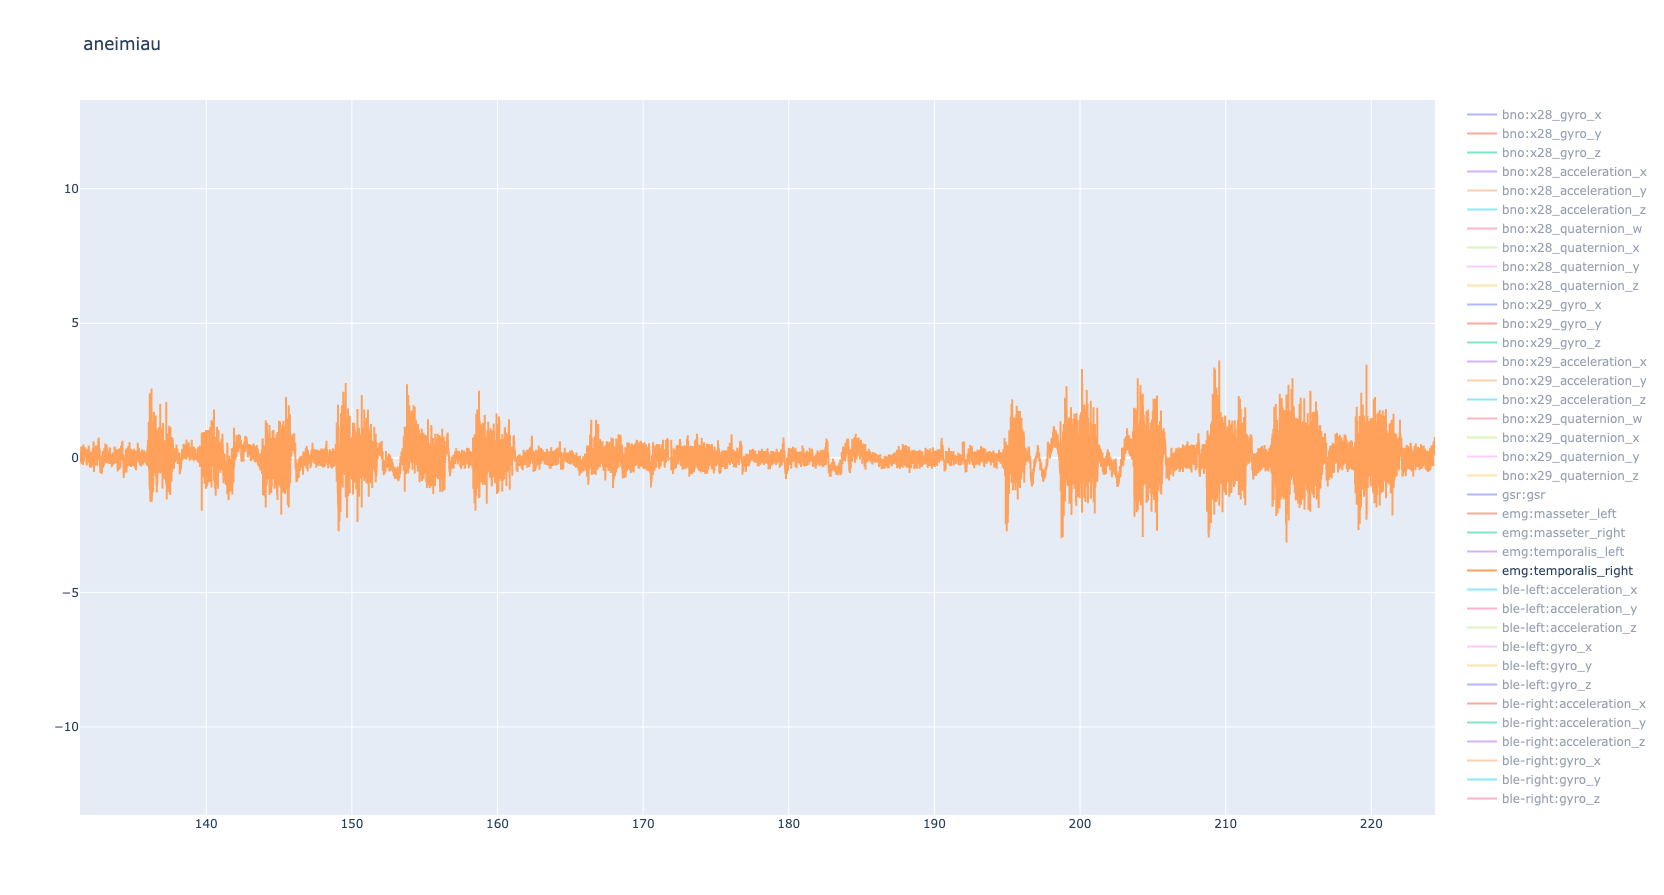
\includegraphics[width=\textwidth]{src/media/study/plots/temporalis_right.png}
\caption{Example of a right temporalis time-series slice. From left to right: 3x2s clenching with the right side; 3x4s clenching with the right side; 3x2s clenching with the front side; 3x4s clenching with the front side; 3x2s clenching with all sides; 3x4s clenching with all sides}
\label{plot:temporalis_right}
\end{sidewaysfigure}

\begin{sidewaysfigure}[h]
\centering
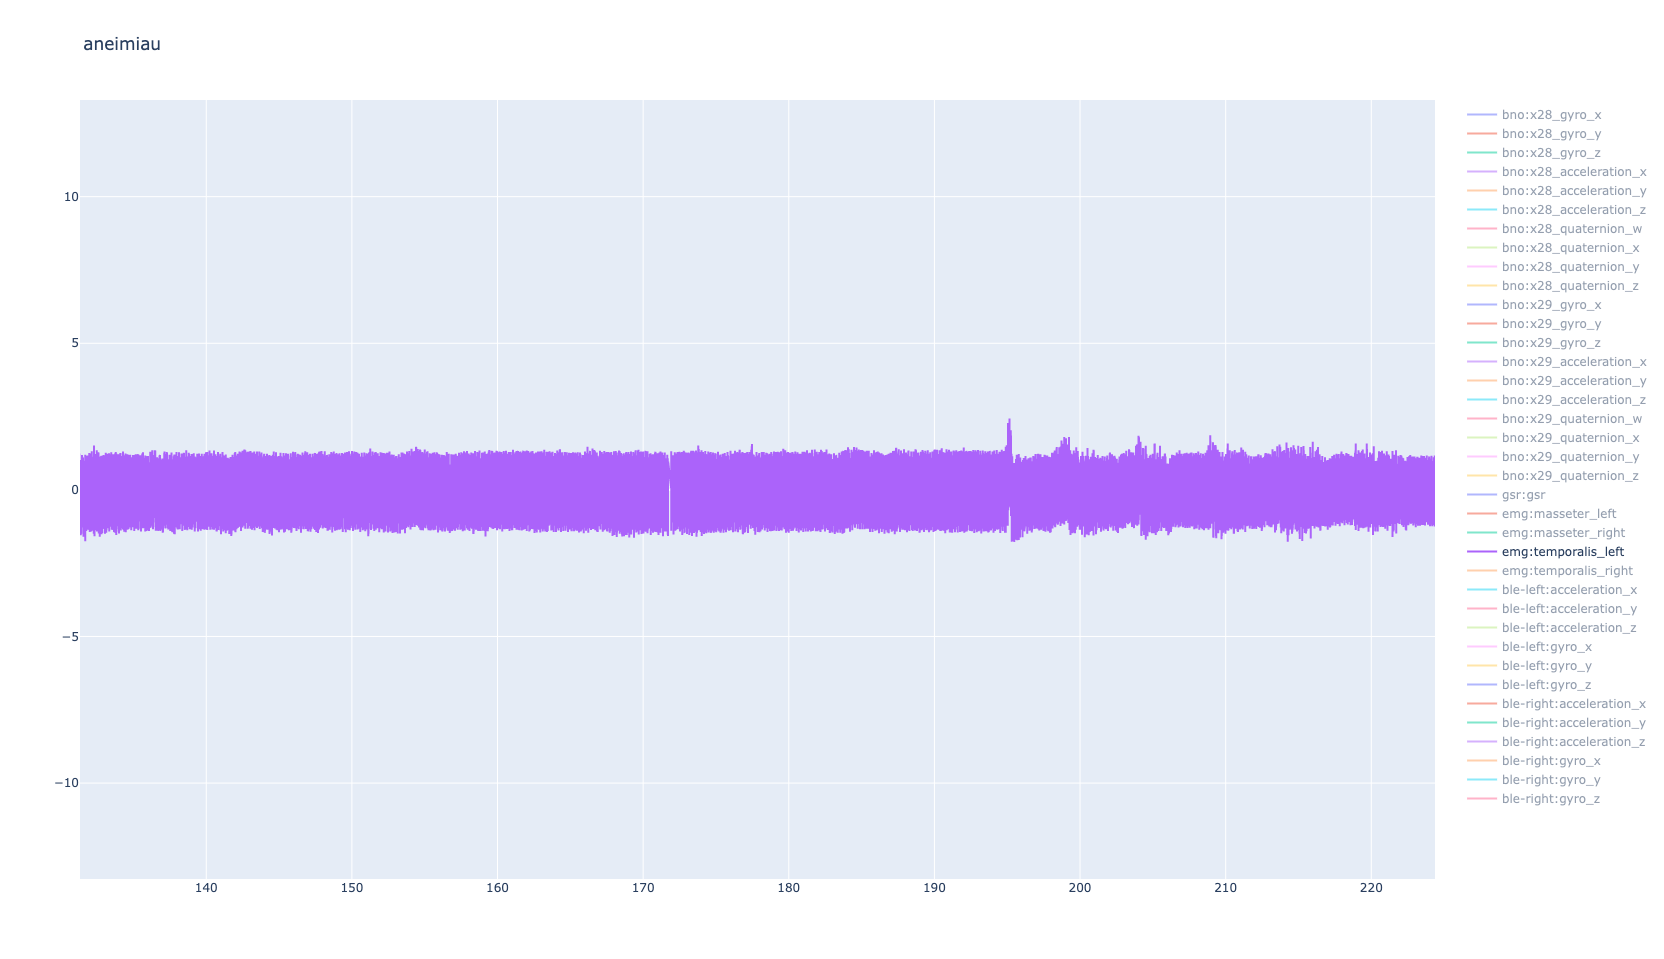
\includegraphics[width=\textwidth]{src/media/study/plots/temporalis_left.png}
\caption{Example of a left temporalis time-series slice. From left to right: 3x2s clenching with the right side; 3x4s clenching with the right side; 3x2s clenching with the front side; 3x4s clenching with the front side; 3x2s clenching with all sides; 3x4s clenching with all sides. Note that it's not possible to differentiate between the performed exercises here.}
\label{plot:temporalis_left}
\end{sidewaysfigure}

\begin{sidewaysfigure}[h]
\centering
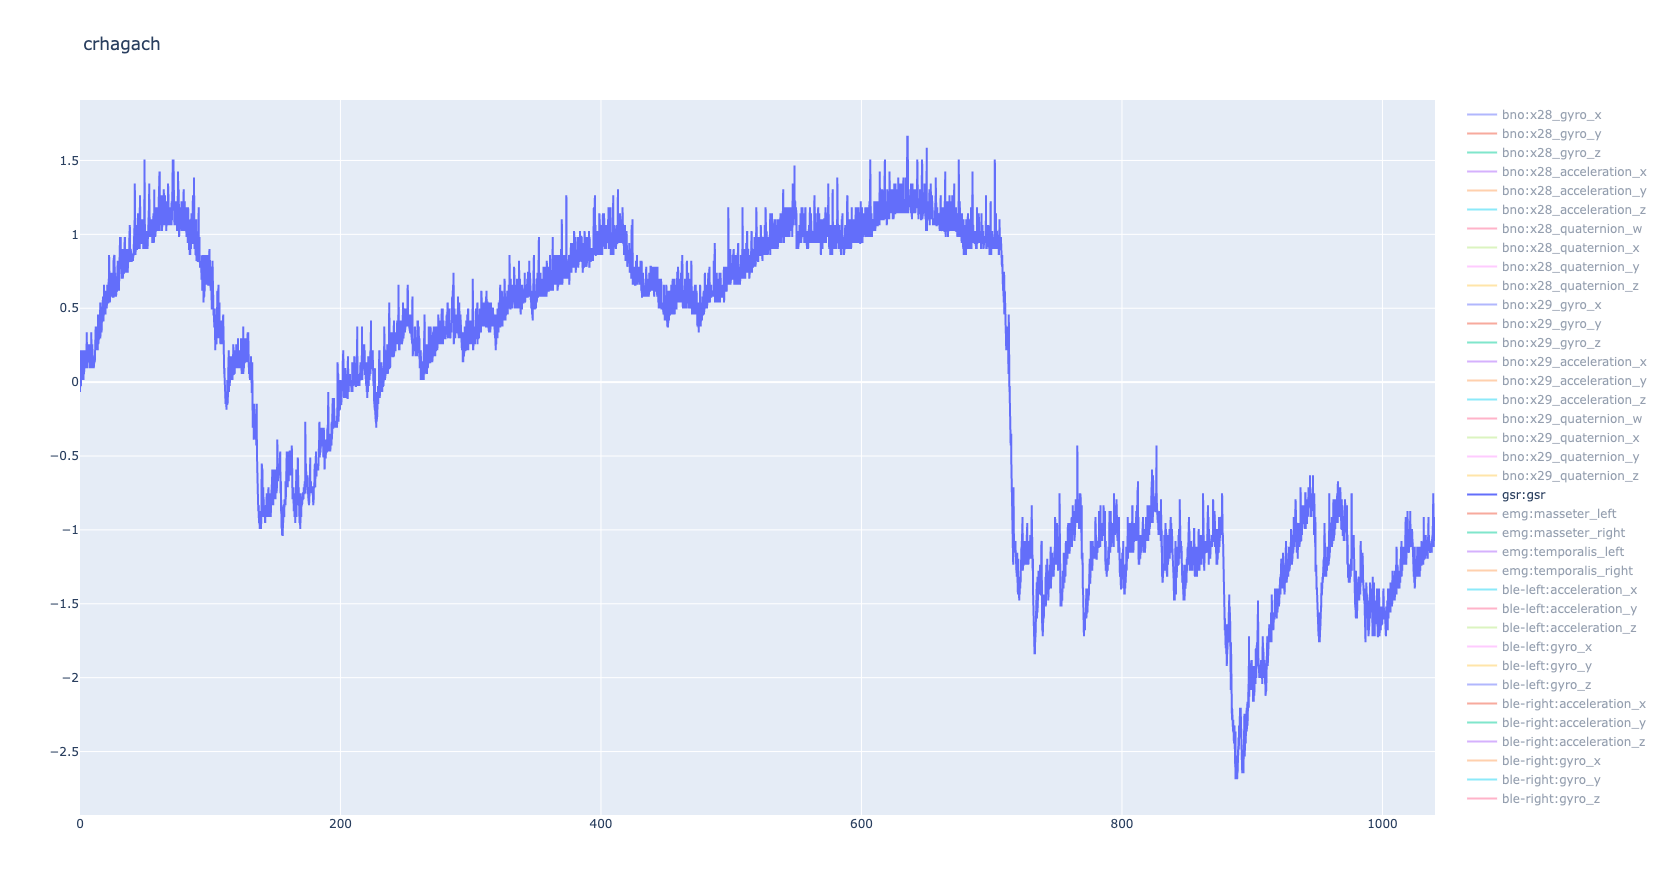
\includegraphics[width=\textwidth]{src/media/study/plots/gsr.png}
\caption{Example of a GSR time-series}
\label{plot:gsr}
\end{sidewaysfigure}

\begin{sidewaysfigure}[h]
\centering
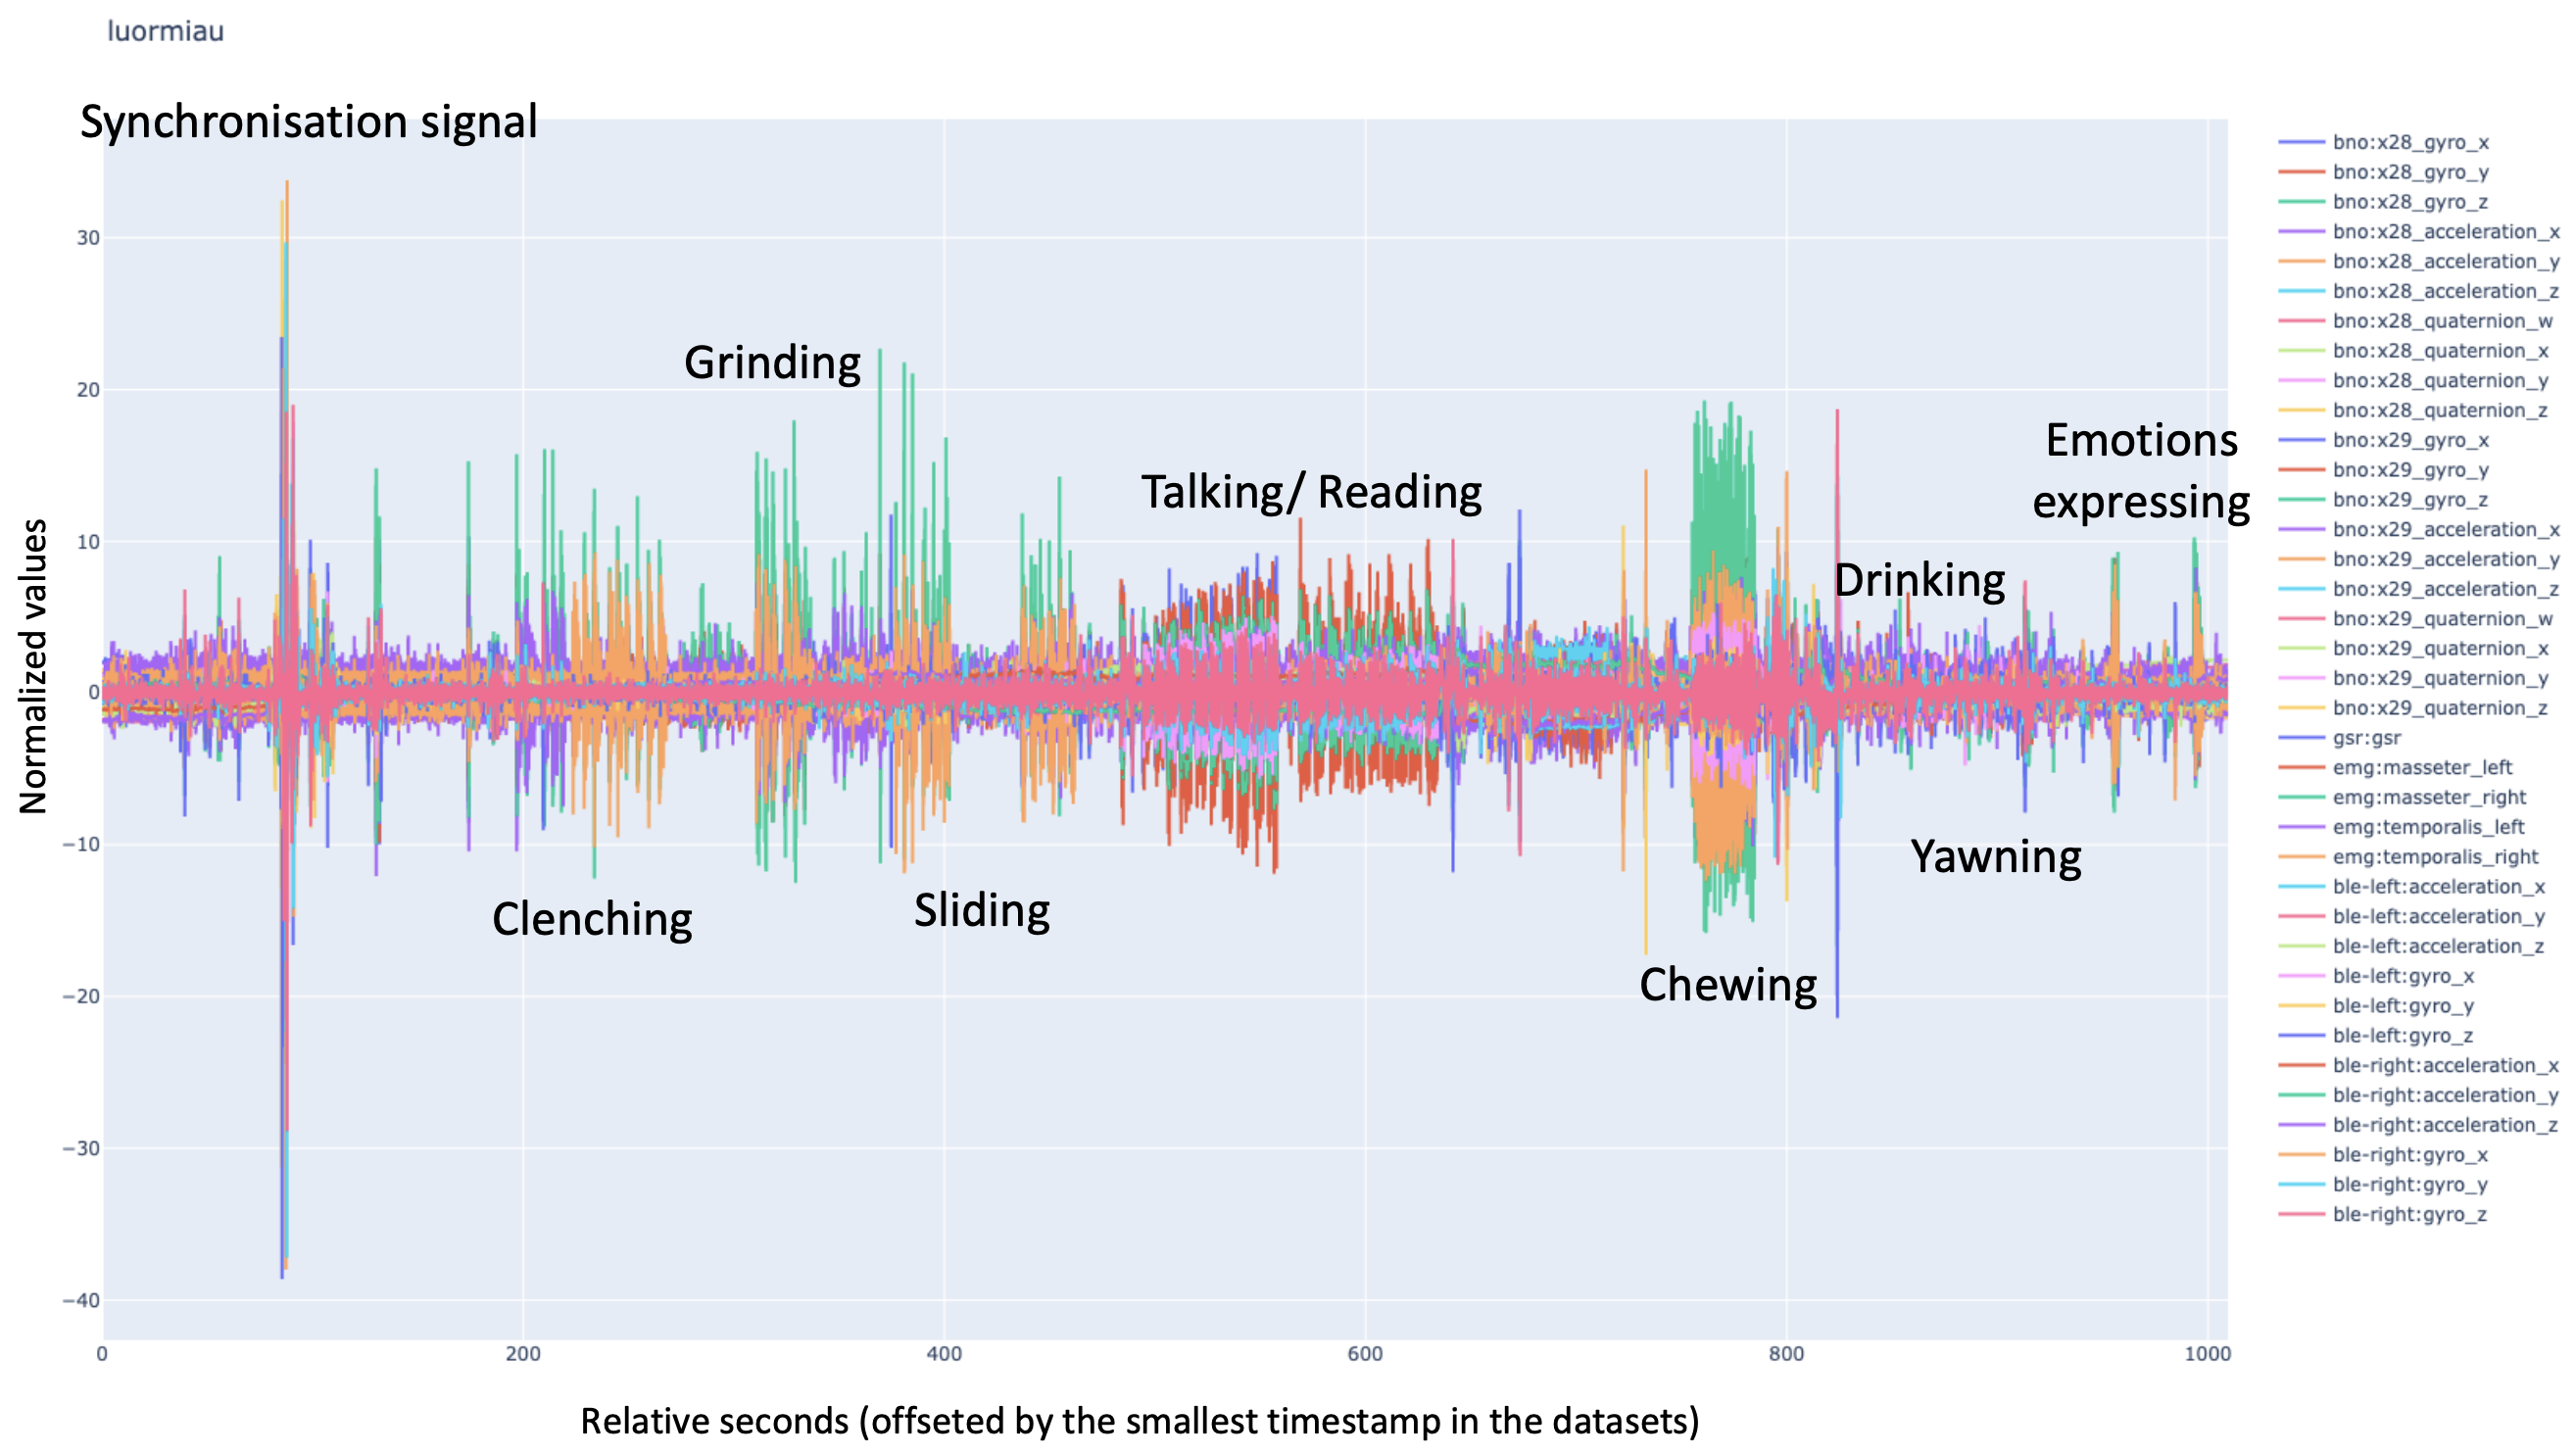
\includegraphics[width=\textwidth]{src/media/methodology/overview.png}
\caption{Overview of a normalized dataset}
\label{image:dataset_overview}
\end{sidewaysfigure}
%\include{src/appendix/anhang_b}

%% --------------------
%% |   Bibliography   |
%% --------------------

\cleardoublepage
\phantomsection
\addcontentsline{toc}{chapter}{\bibname}
\printbibliography

\end{document}
%% --------------------------------------------------------------------------------
%% |                              END OF DOCUMENT                                 |
%% --------------------------------------------------------------------------------